% =============================================================================
%  MYSSP 2026 RESEARCH PAPER -- final report
%  "Seeing Through Solid Rock"
%
%  Compile from this directory with:
%      pdflatex final_report
%      bibtex   final_report
%      pdflatex final_report
%      pdflatex final_report
%
%  The local myssp.sty reproduces the programme header and table style.
%  On Overleaf, replace it with the official MYSSP 2026 myssp.sty if supplied.
% =============================================================================
\documentclass{article}
\usepackage[nonanonymous]{myssp}
\usepackage{hyperref}
\usepackage{booktabs}
\usepackage{amsmath}
\usepackage{xcolor}
\usepackage{graphicx}
\usepackage{subcaption}
\usepackage{siunitx}
\usepackage{float}

\hypersetup{colorlinks=true, linkcolor=blue, citecolor=blue, urlcolor=blue}
\graphicspath{{../figures/}{figures/}}

% -------- SETUP --------
\title{Seeing Through Solid Rock:\\
       A Reproducible Simulation of Muon Radiography for a Hidden Chamber}

\author{%
  \begin{tabular}{c}
  Evan Lim Hong Yan \\
  MYSSP 2026 Participant \\
  Malaysia \\[0.7em]
  Junyi Chai \\
  MYSSP 2026 Participant \\
  Malaysia \\[0.7em]
  Samantha Chan Teng Wei \\
  MYSSP 2026 Participant \\
  Malaysia \\[1.0em]
  Mentor: Assoc.\ Prof.\ Dr.\ Khaw Kim Siang \\
  Muon Physics Group, Tsung-Dao Lee Institute \\
  Shanghai Jiao Tong University, China
  \end{tabular}
}
% -----------------------------------------

\begin{document}

\maketitle

\begin{abstract}
Muography images the interior of a dense object by counting cosmic-ray muons
that survive passage through it. We built a reproducible Python simulation of a
230~m square-based limestone pyramid containing a 10~m radius spherical
chamber, observed by a 0.25~m$^2$ detector with a $\pm40^\circ$ field of view
and $2^\circ$ angular pixels. The simulation combines a measured cosmic-ray
muon spectrum, exact range--energy energy loss, ray-marched opacity, expected
counts, Poisson noise, and two distinct significance definitions. For the
baseline model the expected signal in a fixed direction reaches three standard
deviations ($3\sigma$) after 4.8 days and five standard deviations
($5\sigma$) after 13.4 days; the 30-day expected significance is
$7.50\sigma$. This headline is a deterministic benchmark for the stated model,
not a measurement. Using the exact pixel solid angle lengthens the $5\sigma$
exposure to 15.4 days, a whole-image significance requires about 60 days, and a
4\% error in the assumed rock density can fake a $5\sigma$ signal at 180 days.
All four named parameter studies were completed: chamber radius, chamber
depth, detector placement, and angular binning. A hypothetical Malaysian
limestone hill with an 8~m cave would require about 9 days. The work shows how
geometry, counting statistics, and systematics control the detectability of a
subsurface void, and provides a reproducible template for teaching muon
radiography.

\textbf{Keywords:} cosmic-ray muons, muography, Monte Carlo simulation,
Poisson statistics, exposure optimisation.
\end{abstract}

\section{Introduction}

Every minute, roughly $10^4$ cosmic-ray muons cross every square metre of
ground at sea level. They are produced when high-energy cosmic rays strike
nuclei in the upper atmosphere, creating pions that decay into muons. A muon is
a heavy cousin of the electron: the same charge, about 207 times the mass, and
a rest lifetime of $2.2~\mu$s. A naive calculation says that a muon travelling
at nearly the speed of light should decay after about 660~m, so almost none
should reach the ground from the upper atmosphere. They arrive anyway because
their lifetime is dilated by the relativistic factor $\gamma$; cosmic-ray muons
are one of the most direct everyday demonstrations of special relativity.

The same properties make muons a penetrating probe. In the minimum-ionising
regime a charged particle loses about 2~MeV per gram per square centimetre, so
a muon with tens of GeV can cross tens of metres of rock. A muon is heavy
enough that the radiative loss which stops an electron is suppressed by a
factor of order $207^2$, and it does not feel the strong force that absorbs
protons and alpha particles. The result is a natural X-ray machine the size of
the sky: a detector beside a mountain counts muons from each direction, and a
line of sight with less material transmits more muons than the surrounding
rock \cite{bonomi2020,pdg2024}.

Muography is an old idea. Alvarez et al.\ searched for hidden chambers in the
Pyramid of Khafre in 1970 \cite{alvarez1970}. It became prominent in 2017 when
the ScanPyramids collaboration reported a large void above the Grand Gallery of
Khufu's pyramid, found independently with nuclear emulsion, scintillator and
gas detectors \cite{morishima2017}. Modern reviews describe applications from
volcanoes to blast furnaces and nuclear reactors \cite{bonomi2020}. What is
often missing from introductory treatments is a complete, reproducible
end-to-end calculation that states explicitly how the exposure time is defined,
how expected and observed significances differ, and how large the leading
systematics are. That gap is the motivation for this work.

This paper answers a deliberately narrow question:

\begin{quote}
\emph{Under a simplified, fully specified simulation model, how many days of
exposure does a 0.25~m$^2$ detector need before the expected chamber signal
reaches $5\sigma$?}
\end{quote}

The objective is not to predict the performance of a real detector, nor to
reproduce the ScanPyramids analysis. It is to build a transparent model in
which every assumption can be inspected, to validate the geometry and
statistics against hand calculations, and to quantify how the answer changes
when one parameter at a time is varied. The result is a benchmark and a
teaching tool, and its limitations are stated explicitly in
Section~\ref{sec:discussion}.


\section{Methodology}
\label{sec:method}

\subsection{Approach and tools}

The study is a computational experiment. A three-dimensional density model is
ray-traced to obtain the opacity in 1681 viewing directions, the opacity is
converted to expected muon counts, and the counts are sampled with a Poisson
distribution. The approach is appropriate because the physical quantity of
interest---the exposure at which a small density contrast becomes statistically
significant---is not available analytically for a finite angular grid and a
realistic target shape. A simulation also allows the same geometry to be run
with and without the chamber, which is the reference needed to divide out the
pyramid's shape.

The implementation uses Python 3.11, NumPy 2.x \cite{harris2020numpy},
Matplotlib 3.11 \cite{hunter2007matplotlib}, and Jupyter
\cite{kluyver2016jupyter}. The supplied physics is in
\texttt{code/muography.py}; the student-owned analysis is in
\texttt{code/student\_analysis.py}; all baseline values live in
\texttt{code/project\_config.py}. The reference random seed is 0. The notebooks
and a summary JSON file are listed in Appendix~\ref{app:code}.

\subsection{Target geometry and detector}

The target is a square-based pyramid with base 230~m, height 139~m, and
density $2.5$~g\,cm$^{-3}$. Its half-width at height $z$ is
\begin{equation}
w(z)=115\left(1-\frac{z}{139}\right)~\mathrm{m}.
\label{eq:width}
\end{equation}
The chamber is a sphere of radius 10~m centred at $(0,0,70)$~m, filled with air
at $1.2\times10^{-3}$~g\,cm$^{-3}$. The detector is a 0.25~m$^2$ square at
$(0,-40,3)$~m, with a $\pm40^\circ$ field of view and $2^\circ\times2^\circ$
pixels, giving $41\times41=1681$ directions. Table~\ref{tab:params} lists the
baseline parameters. The detector lies inside the 230~m footprint; in the model
this is interpreted as a detector in an accessible niche or passage at the base,
and the rock between that niche and the outside is not modelled.

\begin{table}[t]
\centering
\caption{Baseline simulation parameters, stored in
\texttt{code/project\_config.py}.}
\label{tab:params}
\small
\begin{tabular}{@{}lll@{}}
\toprule
Parameter & Baseline & Units \\
\midrule
Detector area & 0.25 & m$^2$ \\
Detector position & $(0,-40,3)$ & m \\
Pyramid base / height & 230 / 139 & m \\
Limestone density & 2.5 & g\,cm$^{-3}$ \\
Chamber radius & 10 & m \\
Chamber centre & $(0,0,70)$ & m \\
Angular field & $\pm40$ & degrees \\
Angular bin size & 2 & degrees \\
Ray step & 0.25 & m \\
Reference random seed & 0 & --- \\
\bottomrule
\end{tabular}
\end{table}


\subsection{Ray tracing and expected counts}

For every direction the opacity is
\begin{equation}
\varrho=\int \rho(\mathbf{r})\,d\ell,
\label{eq:opacity}
\end{equation}
evaluated by marching along the ray in 0.25~m steps and summing
$\rho\,\Delta\ell$, with $\Delta\ell$ converted from metres to centimetres. The
camera is a tangent plane: a direction is specified by two pointing angles,
\begin{equation}
\mathbf{d}=\frac{(\tan a_x,\tan a_y,1)}
{\sqrt{1+\tan^2a_x+\tan^2a_y}},
\label{eq:direction}
\end{equation}
so that $\cos\theta=1/\sqrt{1+\tan^2a_x+\tan^2a_y}$. This parameterisation
keeps the angular grid rectangular and makes the zenith angle a direct
function of the two angles.

The energy-loss rate is modelled by
\begin{equation}
\left\langle-\frac{dE}{dX}\right\rangle=a+bE,
\qquad
a=2.0\times10^{-3}~\mathrm{GeV\,g^{-1}cm^2},\quad
b=4.0\times10^{-6}~\mathrm{g^{-1}cm^2},
\label{eq:loss}
\end{equation}
where $X$ is opacity. Solving $dE/dX=-(a+bE)$ gives the exact minimum
survival energy
\begin{equation}
E_{\min}(\varrho)=\frac{a}{b}\left(e^{b\varrho}-1\right).
\label{eq:emin}
\end{equation}
For small $b\varrho$ this reduces to $E_{\min}\approx a\varrho$. At
$\varrho=25{,}000$~g\,cm$^{-2}$ (100~m of limestone), Eq.~\eqref{eq:emin}
gives $52.6$~GeV, 5.2\% above the linear estimate of 50~GeV.

The expected number of muons in one pixel is
\begin{equation}
\mu=\Phi(E_{\min}(\varrho),\theta)\,A\,\Omega\,T,
\label{eq:counts}
\end{equation}
where $\Phi$ is the integrated muon flux above $E_{\min}$, $A$ is the detector
area, $T$ is the exposure time, and $\Omega$ is the pixel solid angle. The flux
uses the Gaisser parametrisation \cite{gaisser1990} with the low-energy
correction of Guan et al.\ \cite{guan2015}. The project uses the small-angle
convention $\Omega\approx(\Delta\theta)^2$, with
$\Delta\theta=2^\circ=3.49\times10^{-2}$~rad. At the signal direction (about
$30^\circ$ from vertical) this overestimates the exact tangent-plane solid
angle by about 13\%, and at the edge of the field by about 23\%; the effect is
treated as a systematic in Section~\ref{sec:results}.

Two maps are always produced: one for the target with the chamber and one for
the twin target with the chamber filled solid. Their ratio
\begin{equation}
R=\frac{\mu_{\rm void}}{\mu_{\rm rock}}
\label{eq:ratio}
\end{equation}
is the reconstructed radiograph. Away from the chamber $R=1$ because the
pyramid's shape cancels; over the chamber $R>1$ because the missing rock
transmits extra muons.

\subsection{Statistical model}

A simulated observation is a Poisson draw from $\mu$. The observed significance
of a count $N$ against a no-chamber expectation $\mu_0$ is
\begin{equation}
S_{\rm obs}=\frac{N-\mu_0}{\sqrt{\mu_0}},
\label{eq:sobs}
\end{equation}
which changes with the random seed. The expected significance compares two
expectation maps:
\begin{equation}
S_{\rm exp}=\frac{\mu_{\rm void}-\mu_{\rm rock}}{\sqrt{\mu_{\rm rock}}}.
\label{eq:sexp}
\end{equation}
This is deterministic for fixed parameters and defines the smooth exposure
curve. Because both the signal and the background scale linearly with $T$,
$S_{\rm exp}\propto\sqrt{T}$.

The official headline uses $S_{\rm exp}$ at a single signal pixel chosen once
from the noiseless maps, at $(a_x,a_y)=(0^\circ,30^\circ)$; the line of sight
to the chamber centre is at
$\tan\theta=40/(70-3)=0.597$, or $\theta=30.8^\circ$. Choosing the brightest
pixel in each noisy map would select upward fluctuations and bias the result.
The image has 1681 pixels, so a noise-only image is expected to contain about
$1681\times1.35\times10^{-3}=2.27$ pixels above $3\sigma$. This look-elsewhere
effect is quantified in Section~\ref{sec:results}. The $5\sigma$ level is the
project's predefined benchmark, not a complete discovery criterion.

The main methodological limitations are that the model is a two-dimensional
radiograph rather than a three-dimensional tomographic inversion, that muon
scattering and detector response are not simulated, and that the rock density
is assumed known exactly. These choices are justified by the project's scope
and are revisited in Section~\ref{sec:discussion}.


\section{Data Collection}
\label{sec:data}

\subsection{Source and structure of the data}

The data in this project are synthetic by design: they are generated by the
simulation rather than measured with a physical detector. This is appropriate
for a controlled study of the exposure question, because the true density
distribution is known exactly and the same geometry can be run with and without
the chamber. It also means that the results test the internal consistency of
the model, not the performance of a real instrument.

Five data products were generated. (i) Two 1681-pixel expectation maps at 1 and
30 days, one with the chamber and one without, from which the clean ratio and
the expected significance are computed. (ii) A primary Poisson observation at 1
and 30 days using reference seed 0. (iii) A null ensemble of 500 independent
30-day observations of the solid pyramid, used to characterise the
look-elsewhere effect. (iv) An ensemble of 500 observations of the chamber
target at 7, 14 and 30 days, used to characterise the fluctuation of a real
measurement around the expected curve. (v) One-parameter scans: chamber radius
(4--20~m), chamber depth (55--110~m), detector distance and lateral offset,
angular bin size (1--5$^\circ$), detector area (0.0625--2~m$^2$), and assumed
rock density (2.3--2.7~g\,cm$^{-3}$). A hypothetical Malaysian limestone hill
provides an additional target.

Each pixel represents one viewing direction, specified by the two pointing
angles $a_x$ and $a_y$ in degrees. The primary arrays are
$41\times41$; the $1^\circ$ binning scan uses $81\times81$. Counts are stored
as floating-point expectations before sampling and as integer Poisson draws
afterwards. Opacities are in g\,cm$^{-2}$, densities in g\,cm$^{-3}$, angles in
degrees internally and radians in the flux functions, and exposure times in
days. All arrays use a common orientation, \texttt{[iy, ix]}, so a map can be
plotted with the angle grids directly.

\subsection{Preparation and bias controls}

No smoothing, interpolation, outlier removal or missing-value imputation is
applied: the simulation produces a complete array by construction. The only
pre-processing step is the choice of the signal pixel, which is made once from
the noiseless 1-day expectation maps and then held fixed for every exposure and
every noise realisation. This avoids the selection bias that would arise from
choosing the brightest pixel in each noisy map. The reference seed is fixed at
0, and every noisy figure states it. Where an ensemble is used, the ensemble
mean and standard deviation are reported rather than a single draw.

The main sources of bias are model assumptions rather than data handling. The
detector is treated as a point inside the target footprint, so the rock between
the assumed niche and the outside is not counted. The $2^\circ$ pixels are
perfectly independent, whereas a real detector has finite angular resolution.
The rock density is assumed to be exactly 2.5~g\,cm$^{-3}$. These assumptions
are quantified in Section~\ref{sec:results} and discussed in
Section~\ref{sec:discussion}. The data are representative only of the stated
model; they are not a sample of a real pyramid.

\subsection{Data and code availability}

The data are reproducible from the notebooks in the repository. A summary of
every number used in this paper is written to
\texttt{figures/results\_summary.json}. The repository contains the simulation
code, the analysis module, the notebooks, and all figures. The reference seed
is 0. Appendix~\ref{app:data} lists the data sources and software;
Appendix~\ref{app:code} maps figures to notebooks.


\section{Analysis}
\label{sec:analysis}

\subsection{Analytical framework and implementation}

The core analysis chain is: opacity map $\rightarrow$ minimum energy
$\rightarrow$ expected counts $\rightarrow$ ratio map $\rightarrow$ expected
significance $\rightarrow$ exposure curve. The two student-owned functions are
\texttt{opacity\_map}, which builds the angular grids and traces one ray per
pixel, and \texttt{expected\_counts}, which applies
Eqs.~\eqref{eq:counts}--\eqref{eq:ratio}. A third helper,
\texttt{counts\_from\_opacity}, reuses a traced geometry for exposure scans;
because counts are exactly proportional to $T$, this introduces no
approximation. The functions are imported by notebooks 03--05, so every
notebook runs from a fresh kernel without relying on variables left in memory.

The expected-significance curve is evaluated at 14 exposures from 1 to 180 days.
The 5$\sigma$ crossing is obtained by linear interpolation between the two
bracketing points; the exact square-root scaling gives a second, independent
estimate. The four parameter studies change one variable at a time. Studies
A--C evaluate the signal along the exact detector-to-chamber-centre ray rather
than at the maximum of a coarse map, which removes a grid-alignment artefact
that otherwise makes the curves jagged at the few-per-cent level. Study D uses
the full map because the angular binning is the variable under study. Log--log
fits are used only to describe the scaling of significance and exposure with
chamber radius.

Uncertainty is handled at two levels. Statistical uncertainty is estimated from
the 500-member ensembles: the standard deviation of the observed significance
at a fixed pixel, and the distribution of the maximum pixel in the null
experiment. Systematic uncertainty is estimated by repeating the baseline
analysis with (i) the exact tangent-plane pixel solid angle, (ii) a range of
assumed rock densities, (iii) a range of detector areas, and (iv) a per-pixel
versus whole-image definition of significance. The headline itself has no
statistical error bar: it is a deterministic property of the expectation maps.

\subsection{Validation}

Table~\ref{tab:validation} lists the checks. The two most important are the ray
step convergence and the no-void control. Halving the step from 0.25~m to
0.125~m changes the opacity map by at most 0.24\% and by 0.07\% on average. The
no-void control is zero to machine precision away from the chamber, which shows
that the difference map isolates the chamber rather than a geometry bug.

\begin{table}[t]
\centering
\caption{Validation checks. The reference is an independent hand calculation,
a control target, or a statistical expectation.}
\label{tab:validation}
\small
\begin{tabular}{@{}p{4.5cm}p{3.1cm}p{3.4cm}p{2.6cm}@{}}
\toprule
Check & Code result & Reference & Agreement \\
\midrule
Integrated flux above 1~GeV & 60.14 & $\approx60$ (Gaisser/PDG) & 0.2\% \\
$E_{\min}$ at 100~m limestone & 52.59~GeV & 52.59~GeV (exact) & exact \\
$E_{\min}$ vs linear rule & 52.59~GeV & 50~GeV (linear) & 5.2\% \\
Central opacity, vertical ray & 21{,}999 & 21{,}913 (geometry) & 0.4\% \\
Chamber opacity deficit & 4{,}935 & 5{,}000 ($2r\rho$) & 1.3\% \\
Ray step 0.25 $\to$ 0.125~m & --- & --- & max 0.24\% \\
No-void control & 0.00 & 0 by construction & exact \\
Clean ratio away from chamber & 1.0000 & 1 by construction & exact \\
Poisson spread at mean 10{,}000 & 100.9 & $\sqrt{10{,}000}=100$ & 0.9\% \\
Null maximum (500 runs) & 3.44 mean & look-elsewhere & see text \\
\bottomrule
\end{tabular}
\end{table}

The hand calculations are reproducible with a calculator. At the chamber the
opacity deficit is $4{,}935$~g\,cm$^{-2}$, against
$2r\rho\times100=5{,}000$ for a 20~m chord; the 1.3\% difference comes from the
discrete ray missing the centre by about 1.3~m. The central vertical opacity is
21,999, against 21,913 from the exact pyramid geometry; the 0.4\% difference is
the 0.25~m marching step. Drawing 5,000 Poisson samples at means 10, 100, 1,000
and 10,000 gives standard deviations 3.2, 9.9, 31.7 and 100.9, compared with
$\sqrt{\mu}=3.16$, 10, 31.6 and 100. The fixed-pixel null distribution has mean
zero and standard deviation about one.


\section{Results}
\label{sec:results}

\subsection{Target and opacity}

Figure~\ref{fig:target} in the Appendix shows the density slice and the opacity
difference produced by the chamber. The raw opacity ranges from $14{,}315$ to
$34{,}993$~g\,cm$^{-2}$, a factor 2.4, because different lines of sight cross
different amounts of the pyramid. The chamber removes $4{,}935$~g\,cm$^{-2}$
along the line of sight, about 19\% of the local opacity and within 1.3\% of
the geometric expectation $2r\rho\times100=5{,}000$ for a 20~m chord. The
no-void control is flat to machine precision away from the chamber. These two
results are the first evidence that the ray tracer and the density model are
correct.

\subsection{Expected counts and the before/after pair}

Figure~\ref{fig:image} shows the 30-day expected-count map and the clean ratio
map. The raw counts run from 191 to 1,197 per pixel, a factor 6.3, and the
total is $9.85\times10^5$ muons. The chamber changes the total by only 0.36\%,
because it affects a small fraction of the image. The raw map is therefore a
picture of the pyramid, not of the chamber.

The clean ratio is 1.0000 away from the chamber and peaks at $1.4758$ at
$(a_x,a_y)=(0^\circ,30^\circ)$. At that pixel the expected counts are 366.8
with the chamber and 248.5 without, an excess of 118.3 muons in 30 days, or
$S_{\rm exp}=7.50\sigma$. The chamber is recovered from the muon data alone,
using the no-void twin as the reference. This ratio map is the ``after'' half
of the before/after pair; the density slice is the ``before'' half.

\begin{figure}[t]
    \centering
    \begin{subfigure}{0.48\textwidth}
        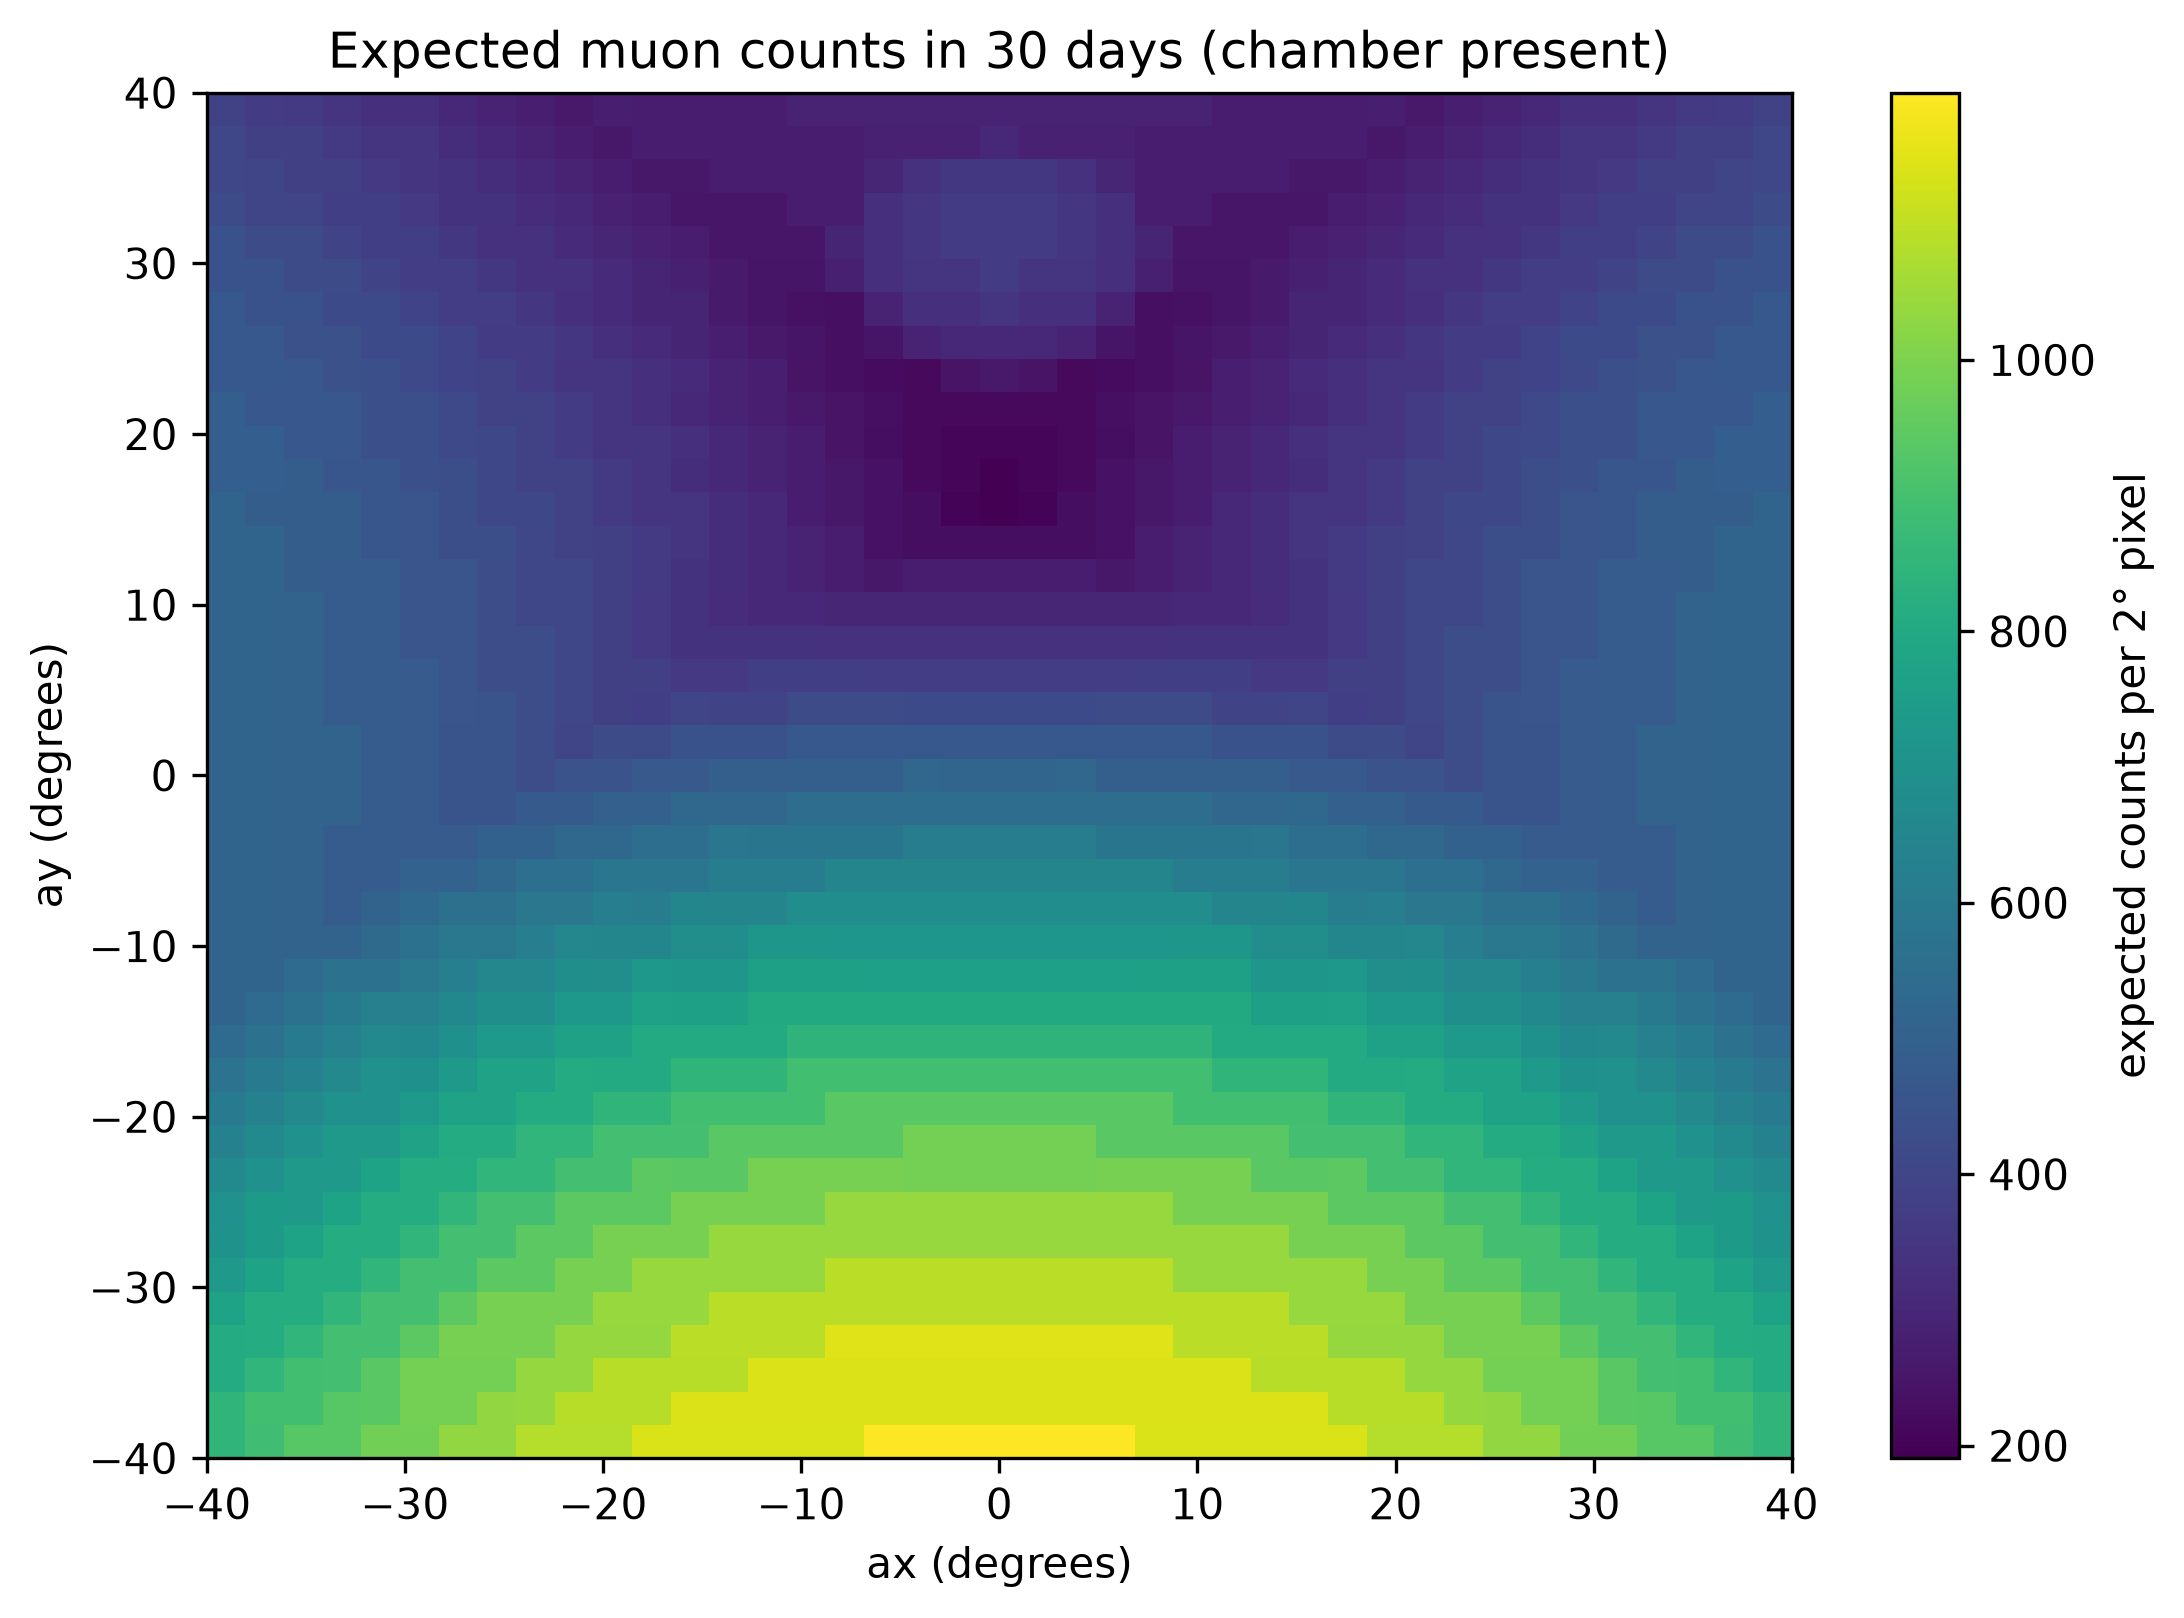
\includegraphics[width=\linewidth]{08_expected_counts.png}
        \caption{Expected counts in 30 days. The pyramid dominates.}
        \label{fig:rawcounts}
    \end{subfigure}\hfill
    \begin{subfigure}{0.48\textwidth}
        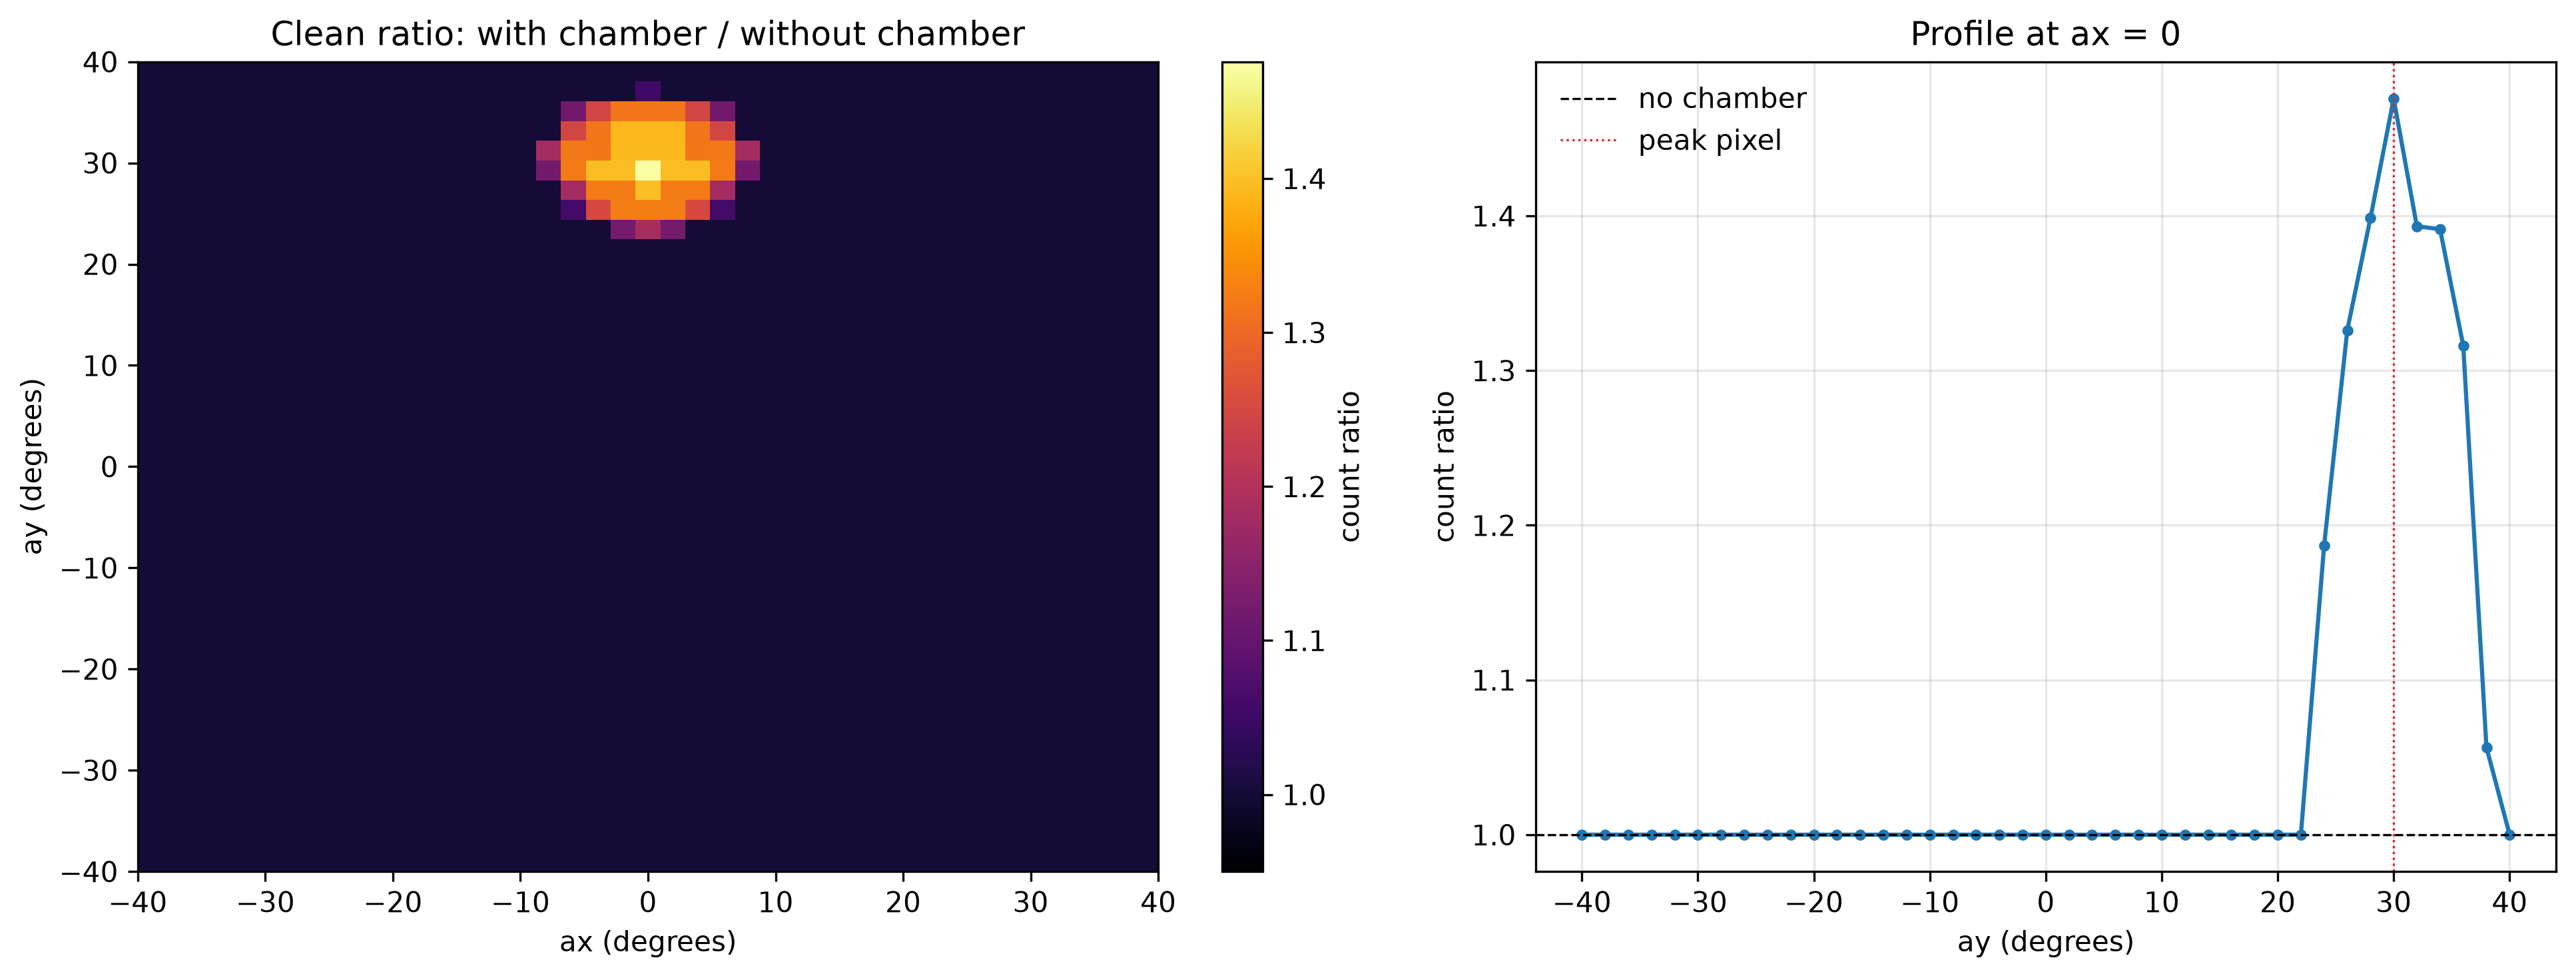
\includegraphics[width=\linewidth]{09_clean_ratio.png}
        \caption{Clean ratio with the no-void twin, and a profile at
        $a_x=0^\circ$. The chamber is the excess above 1.0.}
        \label{fig:ratio}
    \end{subfigure}
    \caption{The before/after pair. The left panel is what the detector counts;
    the right panel is the reconstructed radiograph after dividing out the
    known shape of the pyramid.}
    \label{fig:image}
\end{figure}

\subsection{Noise, observed significance, and the look-elsewhere effect}

Figure~\ref{fig:noise} in the Appendix shows the same analysis after Poisson
sampling with seed 0. At one day the image is noise-dominated: the largest
observed significance is $4.07\sigma$ somewhere by chance, while the fixed
signal pixel is only $1.29\sigma$. At 30 days the chamber is a visible cluster, and the fixed pixel
has observed significance $7.70\sigma$, close to the expected $7.50\sigma$.
The maximum pixel also happens to be $7.70\sigma$ because the signal is real;
at one day the maximum and the fixed pixel are unrelated.

The null control is more informative. In 500 independent 30-day simulations of
the solid pyramid, the largest pixel has mean $3.44\sigma$, median
$3.40\sigma$, and 95th percentile $4.12\sigma$. It exceeds $3\sigma$ in 91.6\%
of images and $5\sigma$ in none. The mean number of pixels above $3\sigma$ is
2.68, close to the naive expectation $1681\times1.35\times10^{-3}=2.27$. A
single $3\sigma$ pixel in a 1681-pixel image is therefore not interesting. This
is the look-elsewhere effect, and it is the reason the headline uses a
pre-selected pixel and the smooth expected curve. The full null distributions
are shown in Appendix Figure~\ref{fig:null}.


\subsection{Exposure curve and the headline result}

The expected significance at the fixed pixel is $1.3696$ after one day. Because
$S_{\rm exp}\propto\sqrt{T}$, the curve in Figure~\ref{fig:exposure} follows
$S(T)=1.3696\sqrt{T/\mathrm{day}}$. It crosses $3\sigma$ at $4.82$ days and
$5\sigma$ at $13.37$ days by linear interpolation; the exact square-root
solution is $13.33$ days. We therefore quote

\begin{quote}
\textbf{For the baseline 0.25~m$^2$ detector and a 10~m radius chamber, the
expected chamber signal reaches $5\sigma$ after approximately 13.4 days under
the project's simplified model.}
\end{quote}

There is no statistical uncertainty on this number: it is a deterministic
property of the model. The red points in Figure~\ref{fig:exposure} show what a
sequence of measurements would look like. At 7 days the mean observed
significance is $3.75\pm1.19$, and 15\% of experiments cross $5\sigma$; at
14 days the mean is $5.12\pm1.24$, and 54\% cross; at 30 days the mean is
$7.53\pm1.23$, and 98\% cross. The expected curve is the average of these
distributions, not a prediction of any one of them. The individual distributions
are shown in Appendix Figure~\ref{fig:dist}.

\begin{figure}[t]
    \centering
    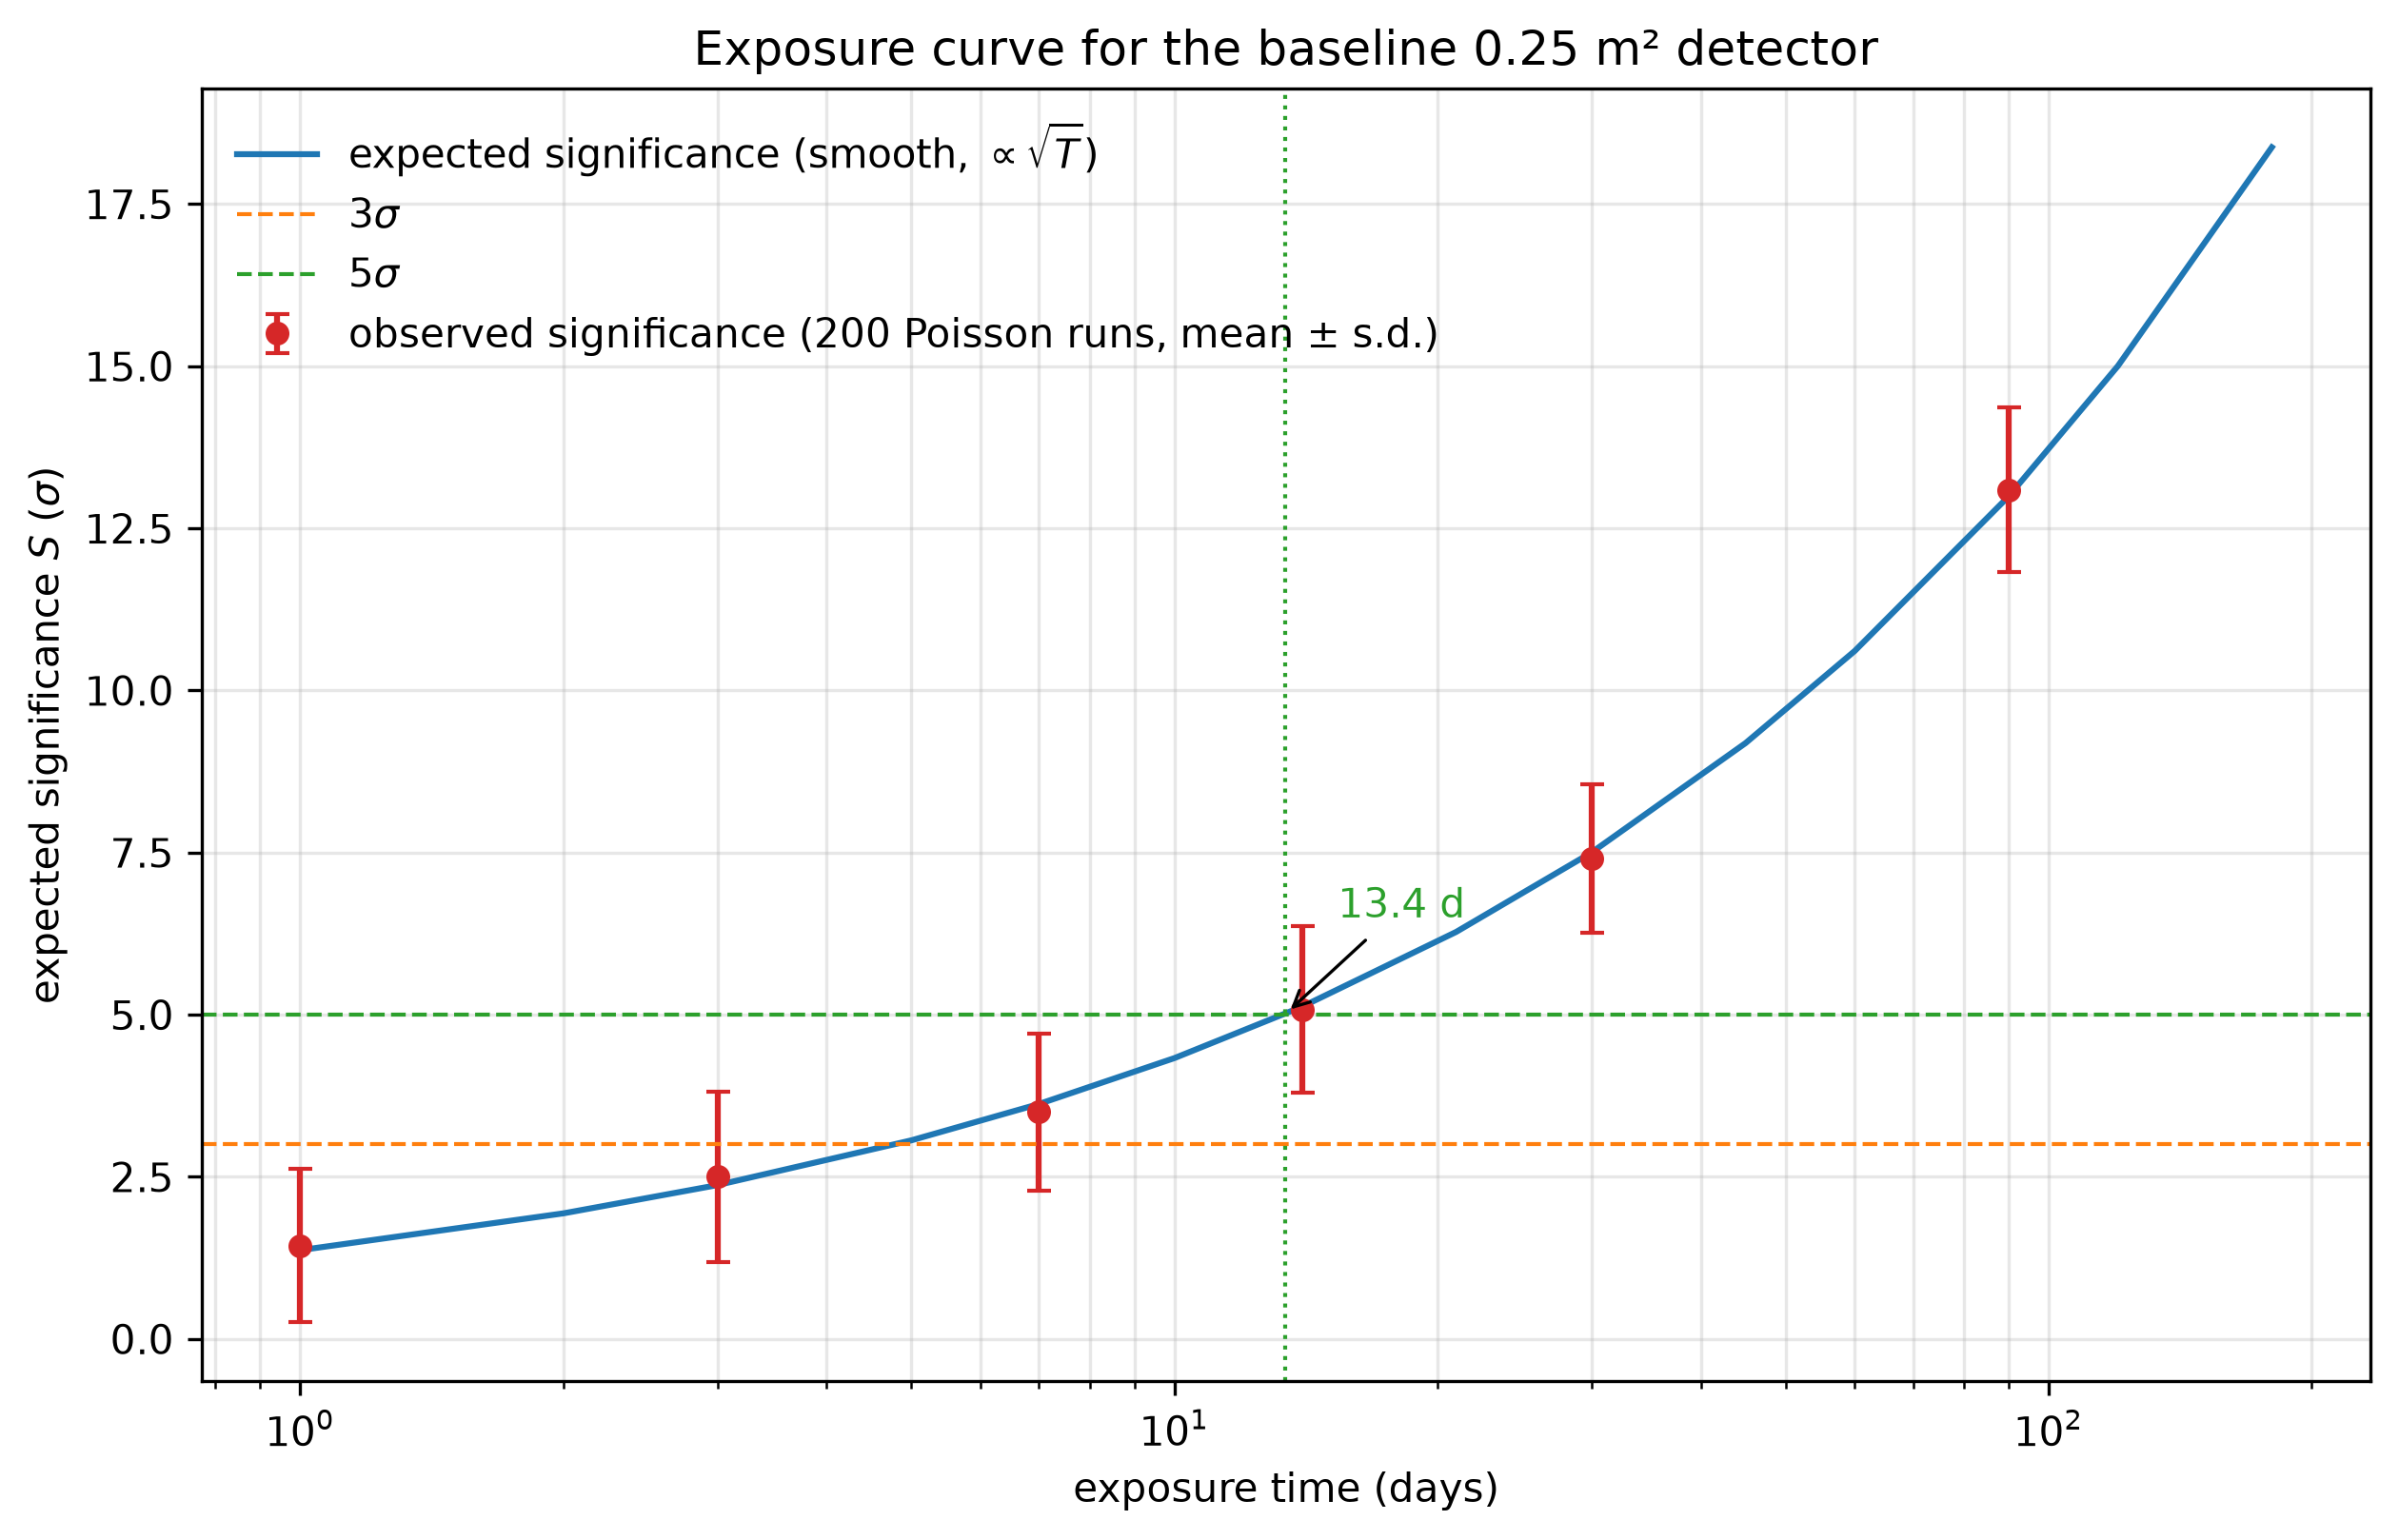
\includegraphics[width=0.64\textwidth]{11_exposure_curve.png}
    \caption{Expected significance versus exposure, with $3\sigma$ and
    $5\sigma$ reference lines. The smooth curve is deterministic; the red
    points are the mean and standard deviation of 200 Poisson experiments at
    selected exposures. The $5\sigma$ crossing is 13.4 days.}
    \label{fig:exposure}
\end{figure}

\subsection{Parameter studies}

All four named studies were completed; Table~\ref{tab:studies} summarises them
and Figure~\ref{fig:studies} shows the results.

\emph{Study A: chamber size.} Varying the radius from 4 to 20~m at fixed depth
and 30 days gives significance from $2.26\sigma$ to $19.43\sigma$ and exposure
from 146.6 to 1.99 days. A log--log fit gives $S\propto r^{1.32}$ and
$T_5\propto r^{-2.65}$. The exponent is close to one, not three: the radiograph
measures the missing chord through the chamber, which grows as $r$, not the
missing volume, which grows as $r^3$.

\emph{Study B: chamber depth.} The accessible range is 55--110~m; below about
52~m the line of sight is outside the $\pm40^\circ$ field. The exposure is
15.4 days at 55~m, rises to 21.6 days at 95~m, and falls to 17.8 days at
110~m. The shallow end has less rock but a larger zenith angle; the deep end
has more rock but a more vertical flux. Above 95~m the chamber approaches the
apex, the ray exits the pyramid soon after the chamber, and the overburden
stops growing.

\emph{Study C: detector placement.} The distance scan has an optimum near
$y=-25$~m, where the exposure is 15.9 days, against 17.3 days at the baseline
$y=-40$~m and 21.7 days at $y=-55$~m. The lateral response is flat within
$\pm30$~m (17.1--19.8 days), with a weak non-monotonicity caused by the line of
sight exiting through different faces of the pyramid.

\emph{Study D: angular binning.} The peak-pixel significance rises from
$3.75\sigma$ at $1^\circ$ to $7.50\sigma$ at $2^\circ$, $12.79\sigma$ at
$4^\circ$ and $18.75\sigma$ at $5^\circ$. This is arithmetic, not physics: the
counts per pixel scale with $\Omega\propto(\Delta\theta)^2$, so
$S_{\rm peak}\propto\Omega/\sqrt{\Omega}\propto\Delta\theta$. The whole-image
significance is almost constant at 3.39--3.61$\sigma$. The coarse-bin ``gain''
is a change in the statistic, not a real gain in detectability. A real detector
would also blur neighbouring directions, which this model does not include.

\begin{table}[t]
\centering
\caption{Summary of the four named parameter studies. Each study changes one
parameter; all others remain at the baseline.}
\label{tab:studies}
\small
\begin{tabular}{@{}p{2.5cm}p{4.0cm}p{5.6cm}@{}}
\toprule
Study & Range & Result \\
\midrule
A: radius & 4--20~m & $T_5$ 146.6 $\to$ 1.99 days; $S\propto r^{1.32}$ \\
B: depth & 55--110~m & $T_5$ 15.4 $\to$ 21.6 $\to$ 17.8 days \\
C: placement & $y=-55$ to $-15$~m & optimum $y\approx-25$~m, 15.9 days \\
D: bin size & $1^\circ$--$5^\circ$ & peak $S$ 3.75 $\to$ 18.75; image $\approx3.5$ \\
\bottomrule
\end{tabular}
\end{table}

\begin{figure}[t]
    \centering
    \begin{subfigure}{0.48\textwidth}
        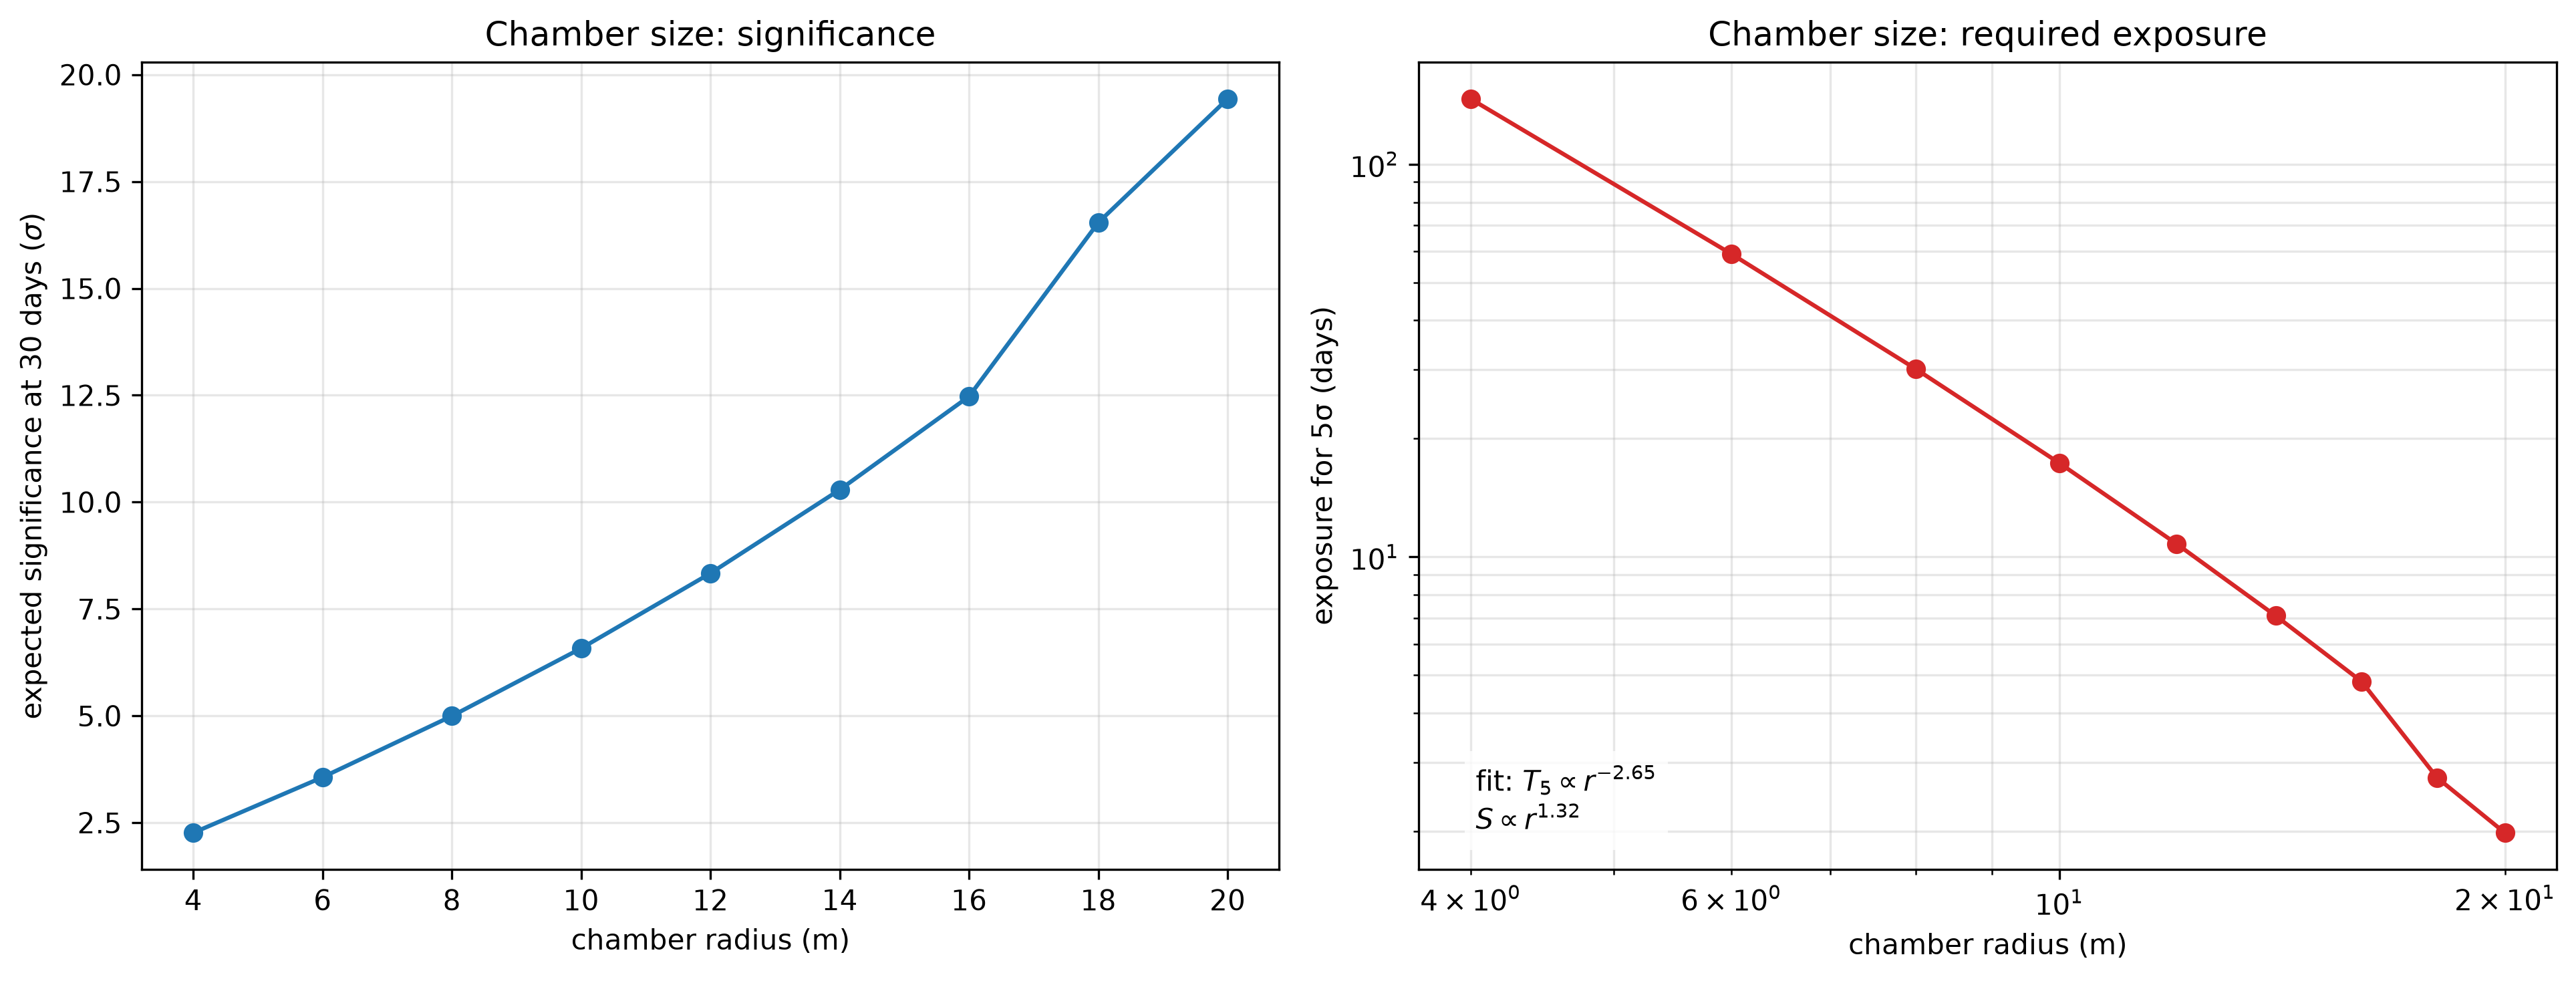
\includegraphics[width=\linewidth]{14_study_A_size.png}
        \caption{Study A: chamber size.}
        \label{fig:studyA}
    \end{subfigure}\hfill
    \begin{subfigure}{0.48\textwidth}
        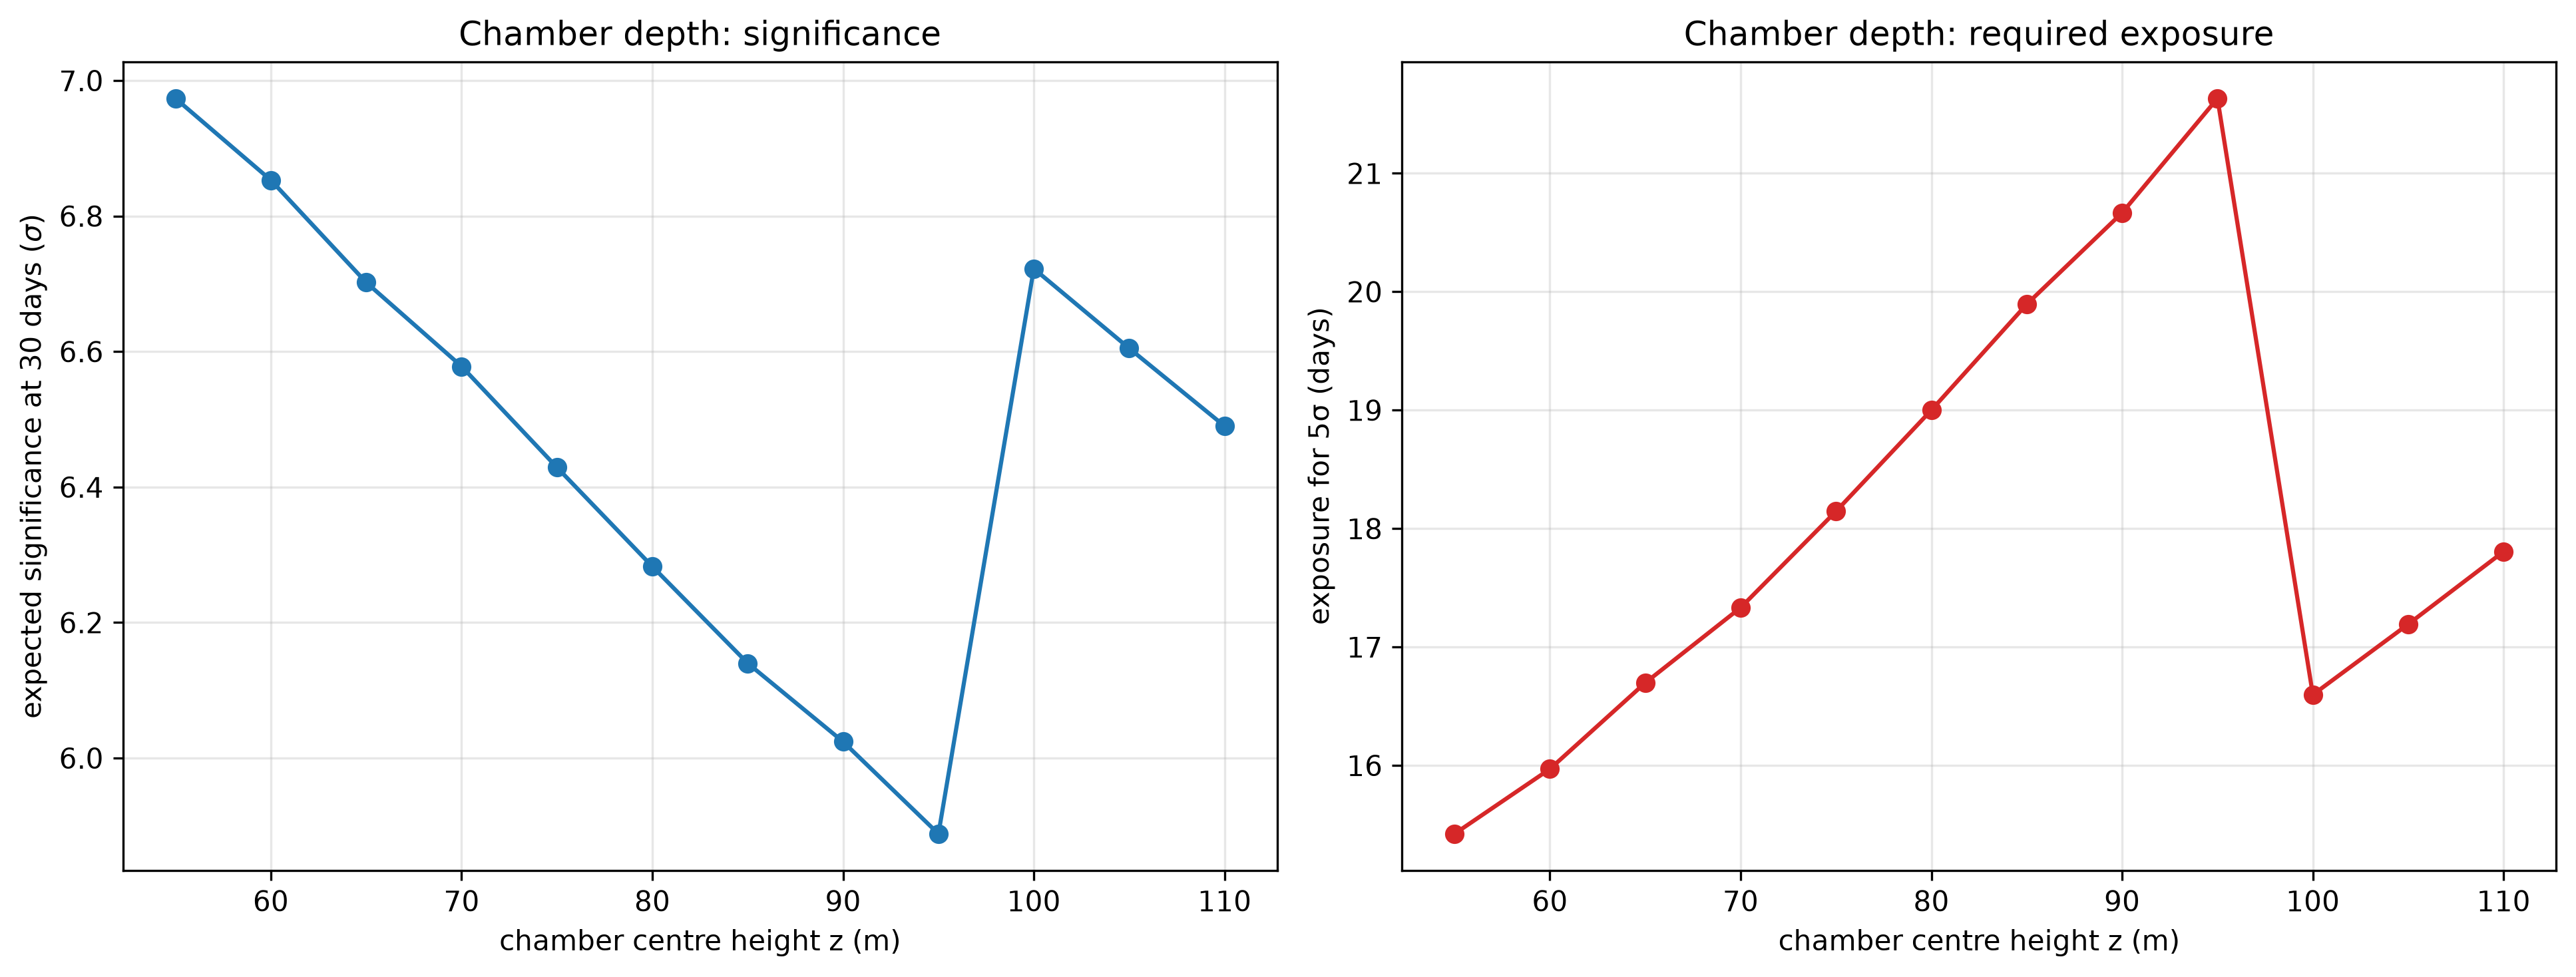
\includegraphics[width=\linewidth]{15_study_B_depth.png}
        \caption{Study B: chamber depth.}
        \label{fig:studyB}
    \end{subfigure}\\[2pt]
    \begin{subfigure}{0.48\textwidth}
        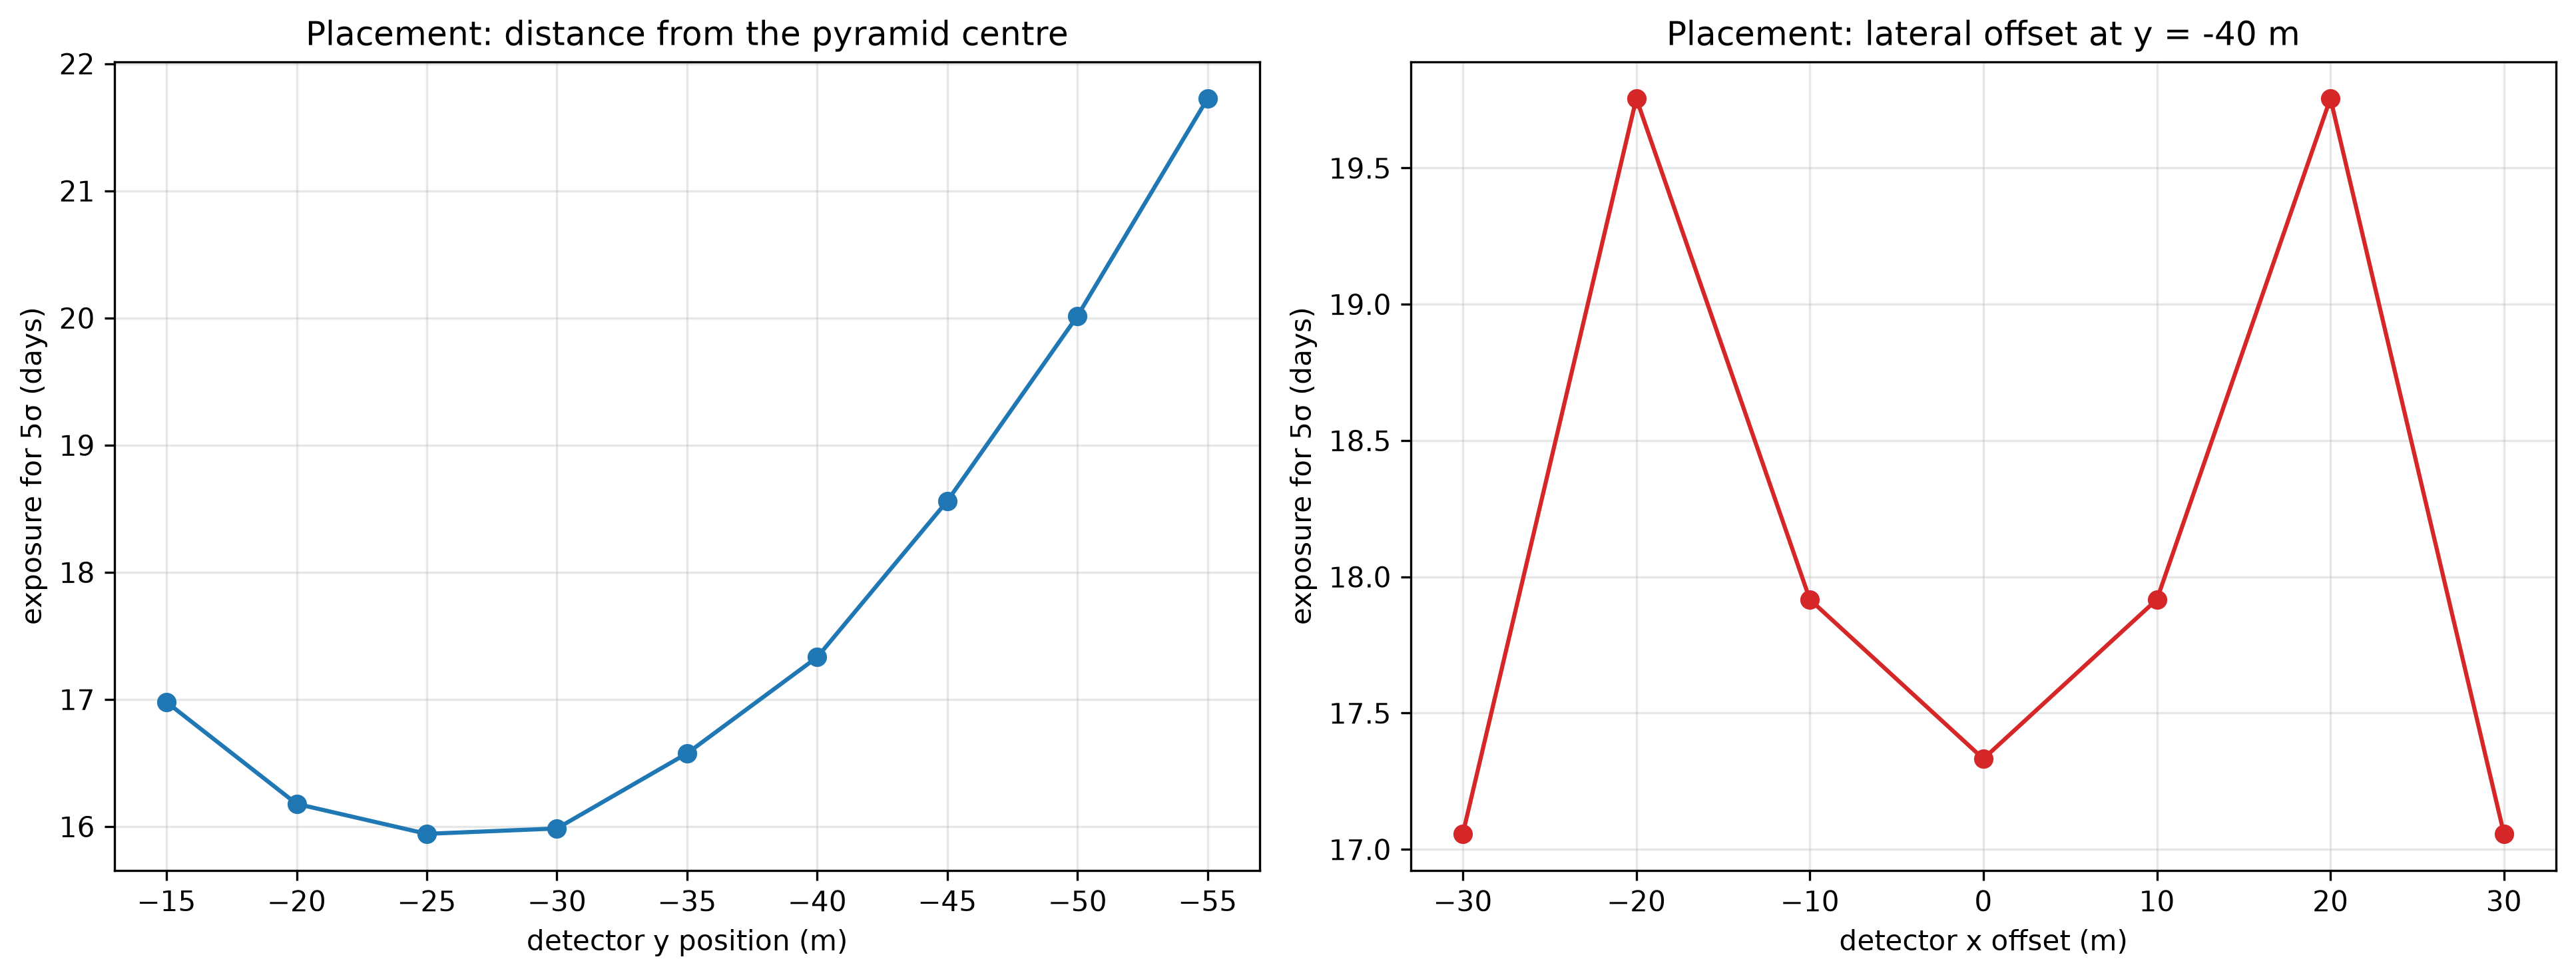
\includegraphics[width=\linewidth]{16_study_C_placement.png}
        \caption{Study C: detector placement.}
        \label{fig:studyC}
    \end{subfigure}\hfill
    \begin{subfigure}{0.48\textwidth}
        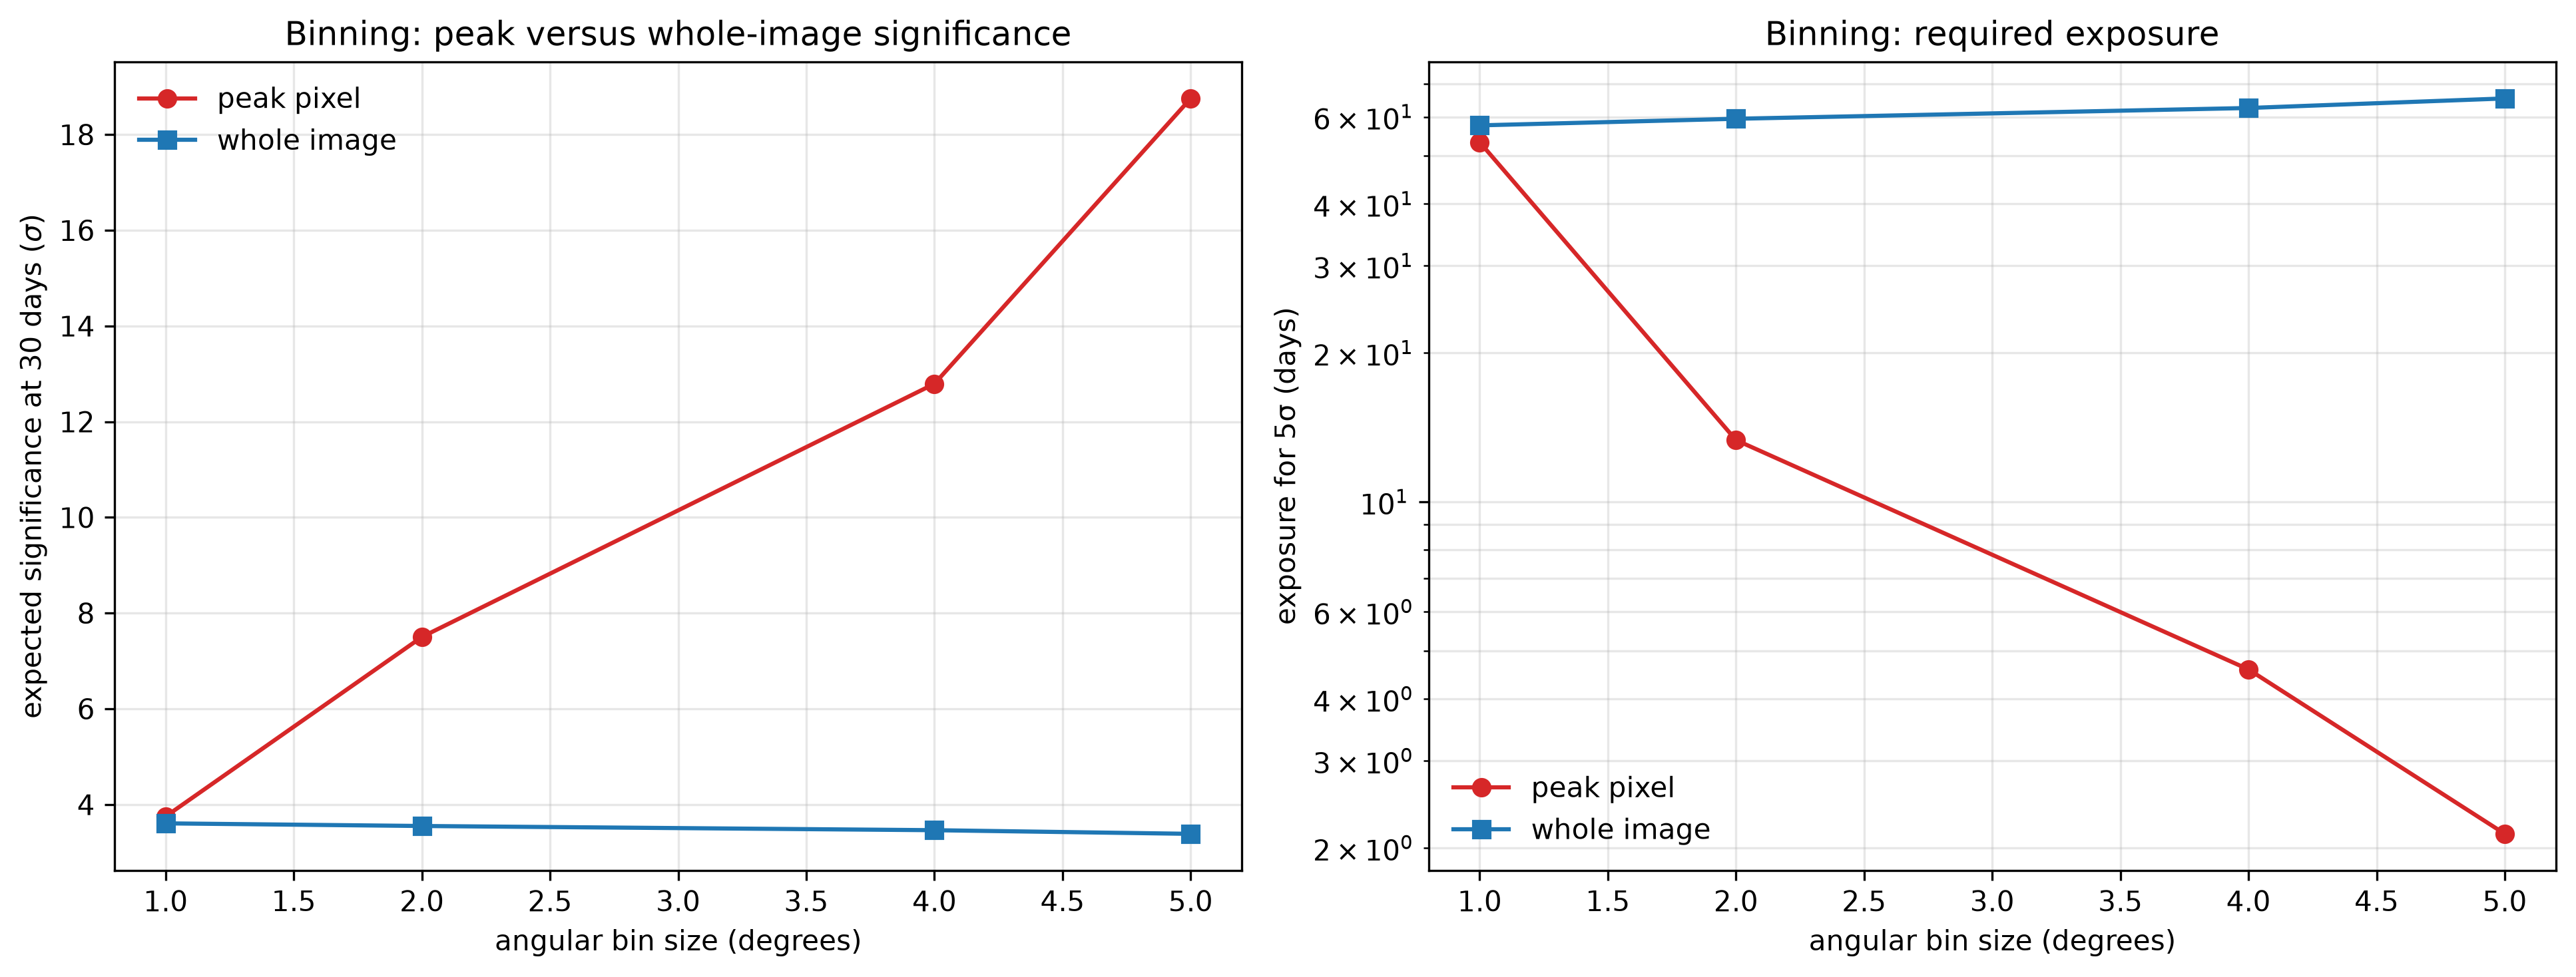
\includegraphics[width=\linewidth]{17_study_D_binning.png}
        \caption{Study D: angular binning.}
        \label{fig:studyD}
    \end{subfigure}
    \caption{The four named parameter studies. Each panel varies one parameter
    at a time and makes one point.}
    \label{fig:studies}
\end{figure}


\subsection{Additional targets and systematics}

Table~\ref{tab:summary} collects the alternative exposure estimates. Using the
exact tangent-plane pixel solid angle instead of the project's small-angle
convention increases the 5$\sigma$ exposure from 13.3 to 15.4 days. The
whole-image statistic, which integrates the excess over all 1681 pixels and
divides by the square root of the total background, gives $3.55\sigma$ at
30 days and a 5$\sigma$ exposure of 59.5 days. Neither is a contradiction: the
per-pixel statistic asks whether one pre-selected direction is bright, while
the whole-image statistic asks whether the total excess is significant.

Detector area scales exactly as expected: $T_5\propto A^{-1.00}$, from
53.3 days at 0.0625~m$^2$ to 1.67 days at 2~m$^2$ (Appendix
Figure~\ref{fig:area}; the observed fluctuation is in
Figure~\ref{fig:dist}). The hypothetical Malaysian limestone hill, with an 8~m
cave seen through about 80~m of rock, reaches $5\sigma$ in 9.1 days (Appendix
Figure~\ref{fig:malaysian}). The most important systematic is the assumed rock
density (Appendix Figure~\ref{fig:densitysys}): analysing a solid target with
2.6 instead of 2.5~g\,cm$^{-3}$ produces a fake maximum of $3.86\sigma$ at
30 days and $9.46\sigma$ at 180 days; at the chamber pixel the fake signal is
$1.11\sigma$ and $2.72\sigma$. With 2.7~g\,cm$^{-3}$ the 180-day maximum is
$14.76\sigma$ and the chamber pixel is $5.36\sigma$. A void and slightly
lighter rock are degenerate in a line-integrated measurement. All estimates are
collected in Table~\ref{tab:summary} and Appendix Figure~\ref{fig:summary}.

\begin{table}[t]
\centering
\caption{Summary of $5\sigma$ exposure estimates under different definitions
and assumptions. The official value is shown in bold.}
\label{tab:summary}
\small
\begin{tabular}{@{}llr@{}}
\toprule
Definition or variation & Note & $T_5$ (days) \\
\midrule
Chamber radius 20~m & Study A & 2.0 \\
\textbf{Baseline, peak pixel} & \textbf{official} & \textbf{13.3} \\
Baseline, exact pixel solid angle & systematic & 15.4 \\
Baseline, whole image (global) & conservative & 59.5 \\
Hypothetical Malaysian hill & 8~m cave & 9.1 \\
Chamber radius 4~m & Study A & 146.6 \\
Detector area 0.0625~m$^2$ & scaling & 53.3 \\
\bottomrule
\end{tabular}
\end{table}


\section{Discussion}
\label{sec:discussion}

The headline is a deterministic benchmark: with the baseline parameters, the
expected signal at one pre-selected direction crosses $5\sigma$ at 13.4 days.
It is not a measurement and it is not a prediction for Khufu. Its value is that
every ingredient is visible: the geometry, the spectrum, the energy-loss model,
the Poisson sampling, and the choice of statistic. The result is therefore
reproducible and can be used to teach why exposure, angular resolution, and
systematics matter.

The result is model-dependent in four important ways. First, detector
acceptance and efficiency are absent; the simulation counts every muon in every
pixel. A 50\% efficient detector doubles the exposure. Second, backgrounds are
absent: electrons from local radioactivity and muons scattered in from outside
the target would add counts that are not modelled. Third, the atmospheric muon
flux varies with pressure and temperature; a real campaign must monitor and
correct it. Fourth, and most important, the rock density is assumed known. A
4\% error already produces a fake $3.86\sigma$ maximum at 30 days and a fake
$9.46\sigma$ maximum at 180 days. Muography measures density along a line, so a
void and slightly lighter rock are degenerate unless an independent density
constraint is available.

The look-elsewhere effect is a second, statistical limitation. A solid pyramid
produces a $3\sigma$ pixel in 91.6\% of 30-day images because the image has
1681 pixels. The project handles this by fixing the signal pixel from the
noiseless model and by reporting the null distribution. A real analysis would
go further and quote a global $p$-value or a trials factor. The $5\sigma$ level
used here is a project benchmark, not a discovery criterion.

The comparison with the 2017 Khufu measurement is at the level of physics and
scale, not a reproduction of the analysis. The ScanPyramids collaboration found
a large void above the Grand Gallery with three independent detector
technologies \cite{morishima2017}. Their measurement faced the same basic
physics as this simulation, but also detector acceptance, efficiency, angular
resolution, backgrounds, and a real, non-uniform target. A roughly 10~m void
inside a roughly 100~m rock target is a several-$\sigma$ measurement only with
a long exposure and careful control of systematics, exactly as the 2017 result
showed.

The limitations of this study are clear. It is a two-dimensional radiograph,
not a three-dimensional tomographic inversion. Muon scattering, detector
response, backgrounds, and atmospheric variation are not simulated. The
detector is an idealised point inside the target footprint, the pixel solid
angle uses a small-angle approximation, and the rock density is fixed. The
study also uses synthetic data by design, so it tests the consistency of the
model rather than the performance of a real instrument.

Several specific next steps follow. A detector-response model with efficiency,
angular resolution, and a point-spread function would show how the chamber
signal is diluted by real binning. A Monte Carlo over rock density and detector
efficiency would turn the single-point systematics into a confidence interval.
A full 3D inversion using several detector positions would move from a
radiograph to a density model. Finally, a real digital elevation model of a
Malaysian limestone hill would replace the conical toy target and make the
stretch estimate directly useful.

\section{Conclusion}

We built a reproducible end-to-end simulation of muon radiography for a
230~m limestone pyramid with a 10~m radius hidden chamber, including ray
tracing, expected counts, Poisson noise, significance, null controls, and four
parameter studies. Under the baseline model the expected chamber signal reaches
$3\sigma$ after 4.8 days and $5\sigma$ after 13.4 days; the 30-day expected
significance is $7.50\sigma$. The answer is controlled by geometry and
statistics rather than by the muon flux alone: the signal follows the missing
chord, the look-elsewhere effect makes a single $3\sigma$ pixel unsurprising,
and a 4\% density error can fake a $5\sigma$ signal at long exposure. The main
limitations are the absence of detector response, scattering, backgrounds,
atmospheric variation, and a full 3D inversion. The most useful next steps are
a detector-response model, a density Monte Carlo, and a tomographic inversion
with multiple detector positions.

\begin{ack}
We thank Assoc.\ Prof.\ Dr.\ Khaw Kim Siang and the Muon Physics Group at the
Tsung-Dao Lee Institute, Shanghai Jiao Tong University, for the project
framework, the supplied physics toolkit, and continuous guidance. We thank the
Malaysia Science Scholars' Programme for the opportunity and support.
\end{ack}



\bibliographystyle{unsrt}
\bibliography{references}

\appendix
\section*{Appendix}

\section{Data Sources and Software}
\label{app:data}

\begin{sloppypar}
This project uses synthetic data generated by the simulation; no external
observational dataset was used. The primary inputs are the baseline parameters
in \texttt{code/project\_config.py}, the supplied physics in
\texttt{code/muography.py}, and the target definition in the notebooks. The
software environment is Python 3.11 with NumPy 2.4 \cite{harris2020numpy},
Matplotlib 3.11 \cite{hunter2007matplotlib}, and Jupyter
\cite{kluyver2016jupyter}. The reference seed is 0. All generated data are
reproducible by running notebooks 02--05 in order; the summary of every number
used in this paper is in \texttt{figures/results\_summary.json}.
\end{sloppypar}

\section{Additional Figures}
\label{app:extra}

\begin{figure}[h]
    \centering
    \begin{subfigure}{0.48\textwidth}
        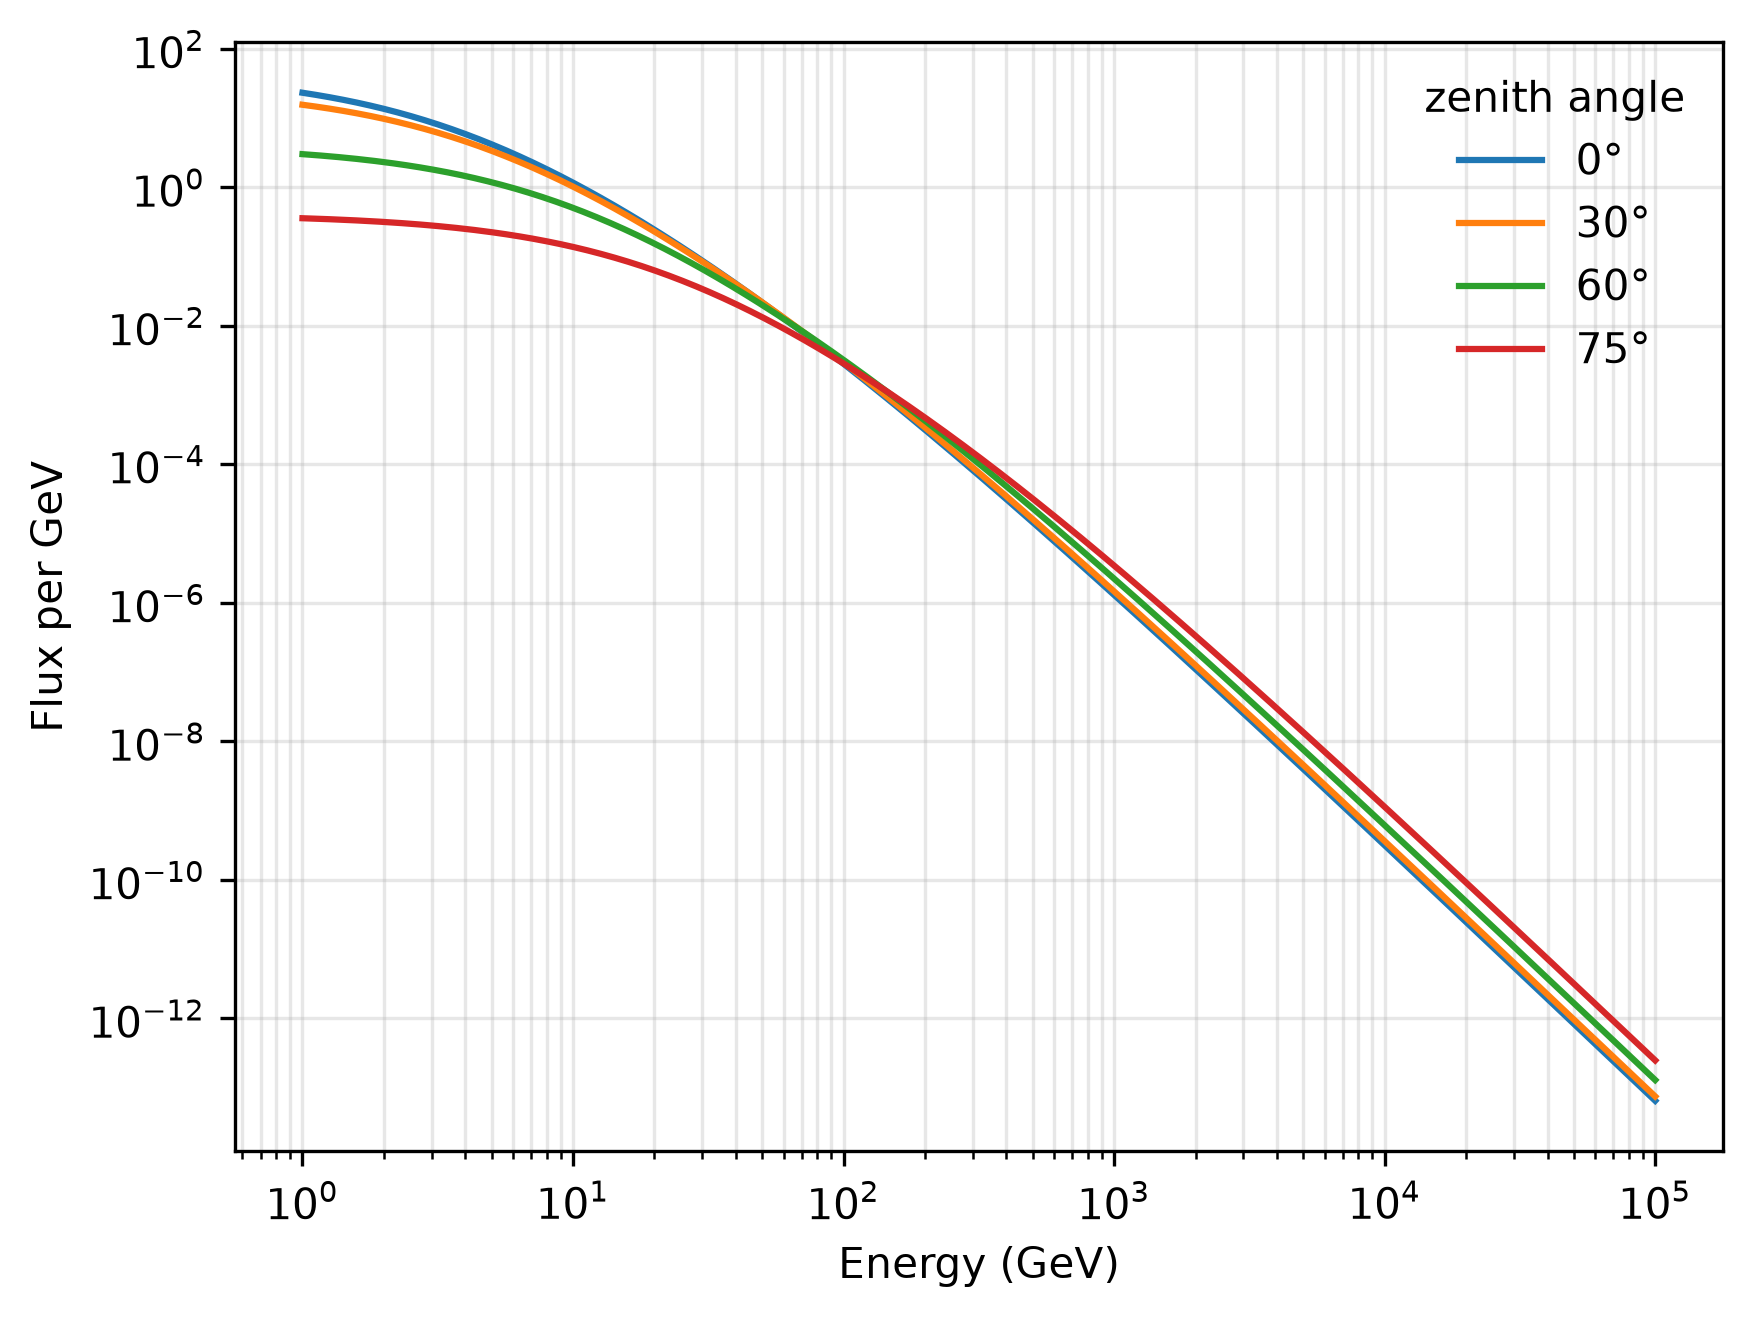
\includegraphics[width=\linewidth]{01_spectrum_angles.png}
        \caption{Differential muon flux at four zenith angles. The spectrum is
        harder at large angles because low-energy muons are removed by the
        longer atmospheric path.}
        \label{fig:spectrum}
    \end{subfigure}\hfill
    \begin{subfigure}{0.48\textwidth}
        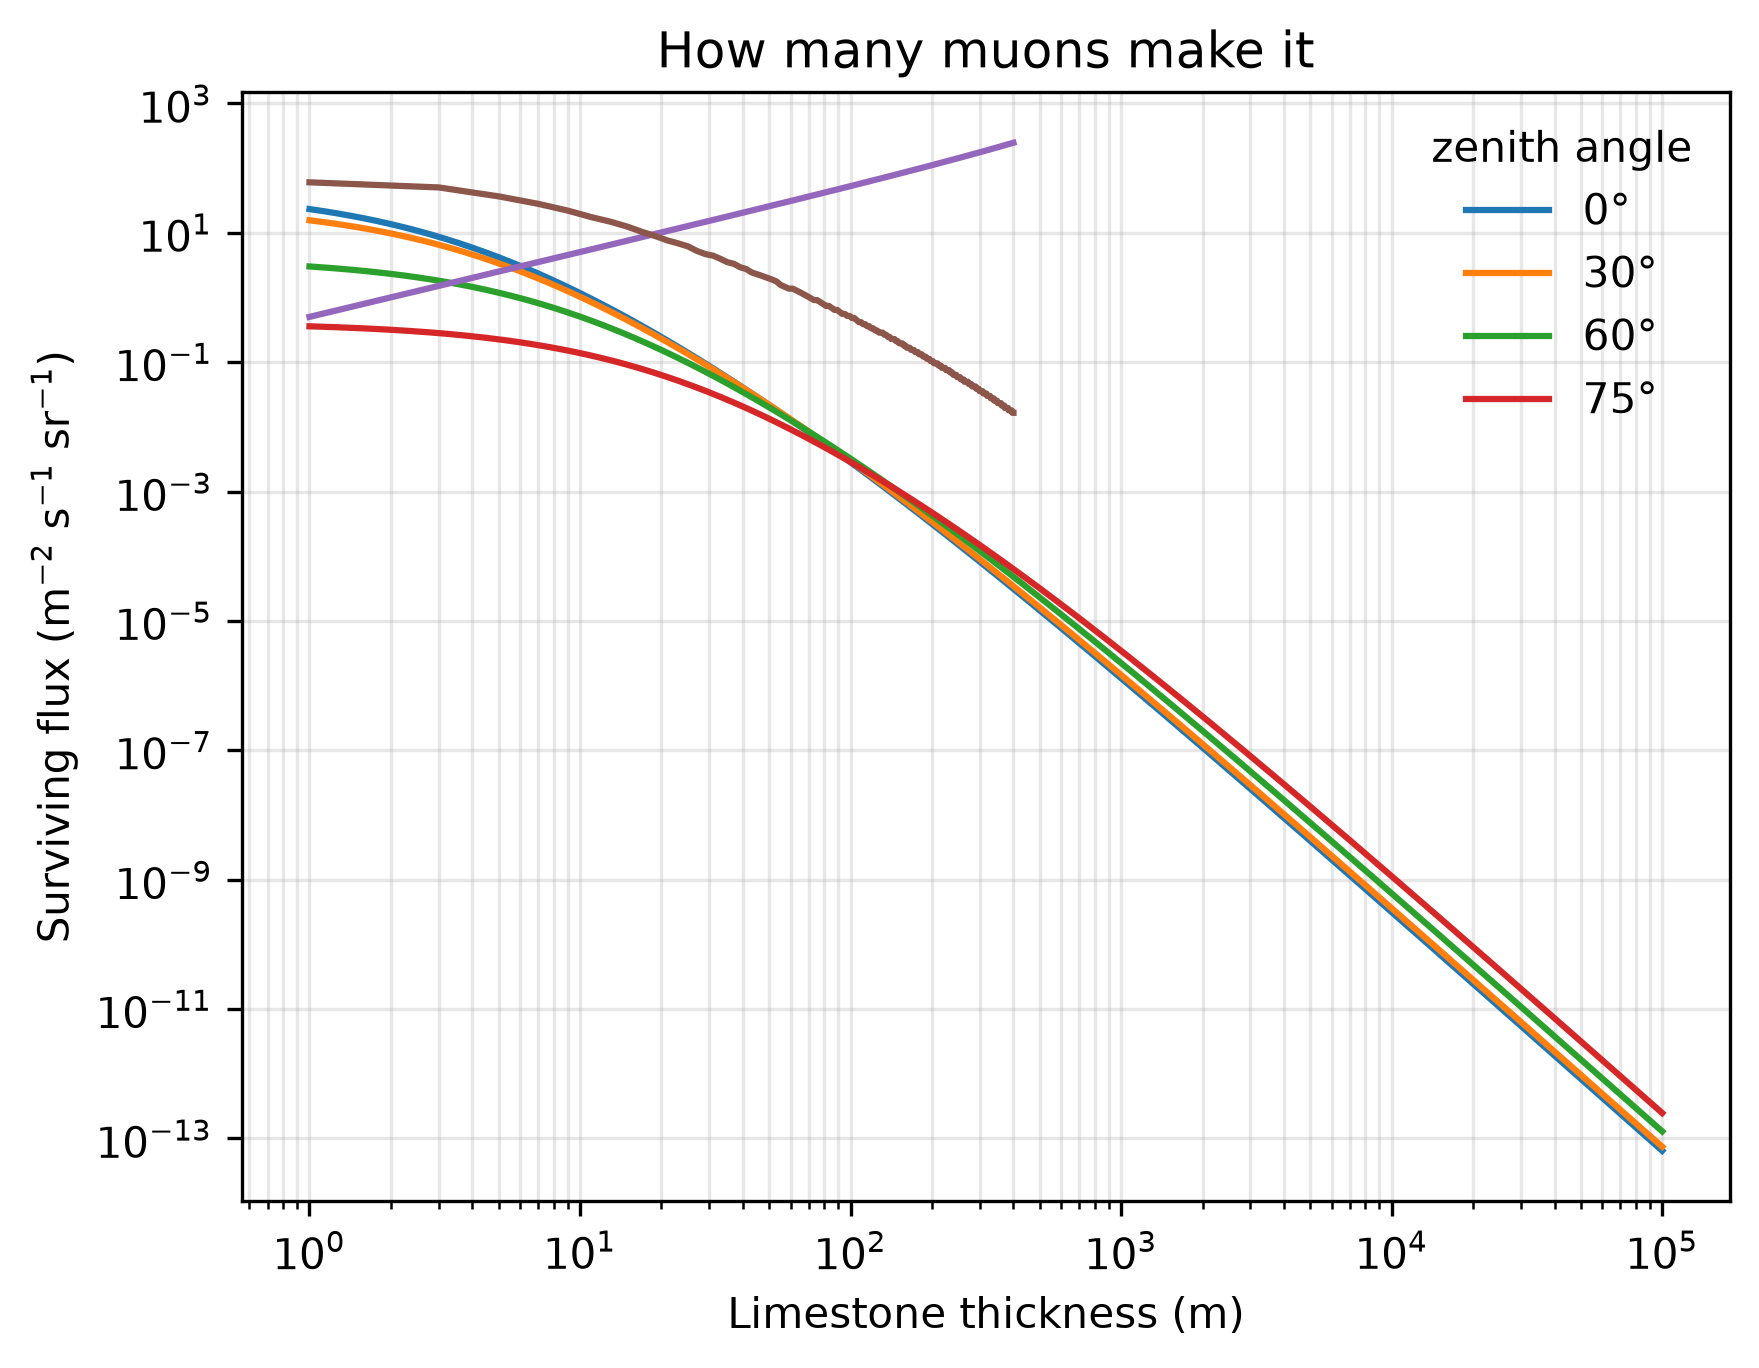
\includegraphics[width=\linewidth]{04_surviving_flux.png}
        \caption{Transmitted flux above the minimum energy through increasing
        limestone thickness; the vertical scale is logarithmic.}
        \label{fig:survival}
    \end{subfigure}
    \caption{The two physics ingredients used by the simulation. Both panels
    are produced by \texttt{notebooks/01\_muons\_and\_rock.ipynb}.}
    \label{fig:physics}
\end{figure}

\begin{figure}[h]
    \centering
    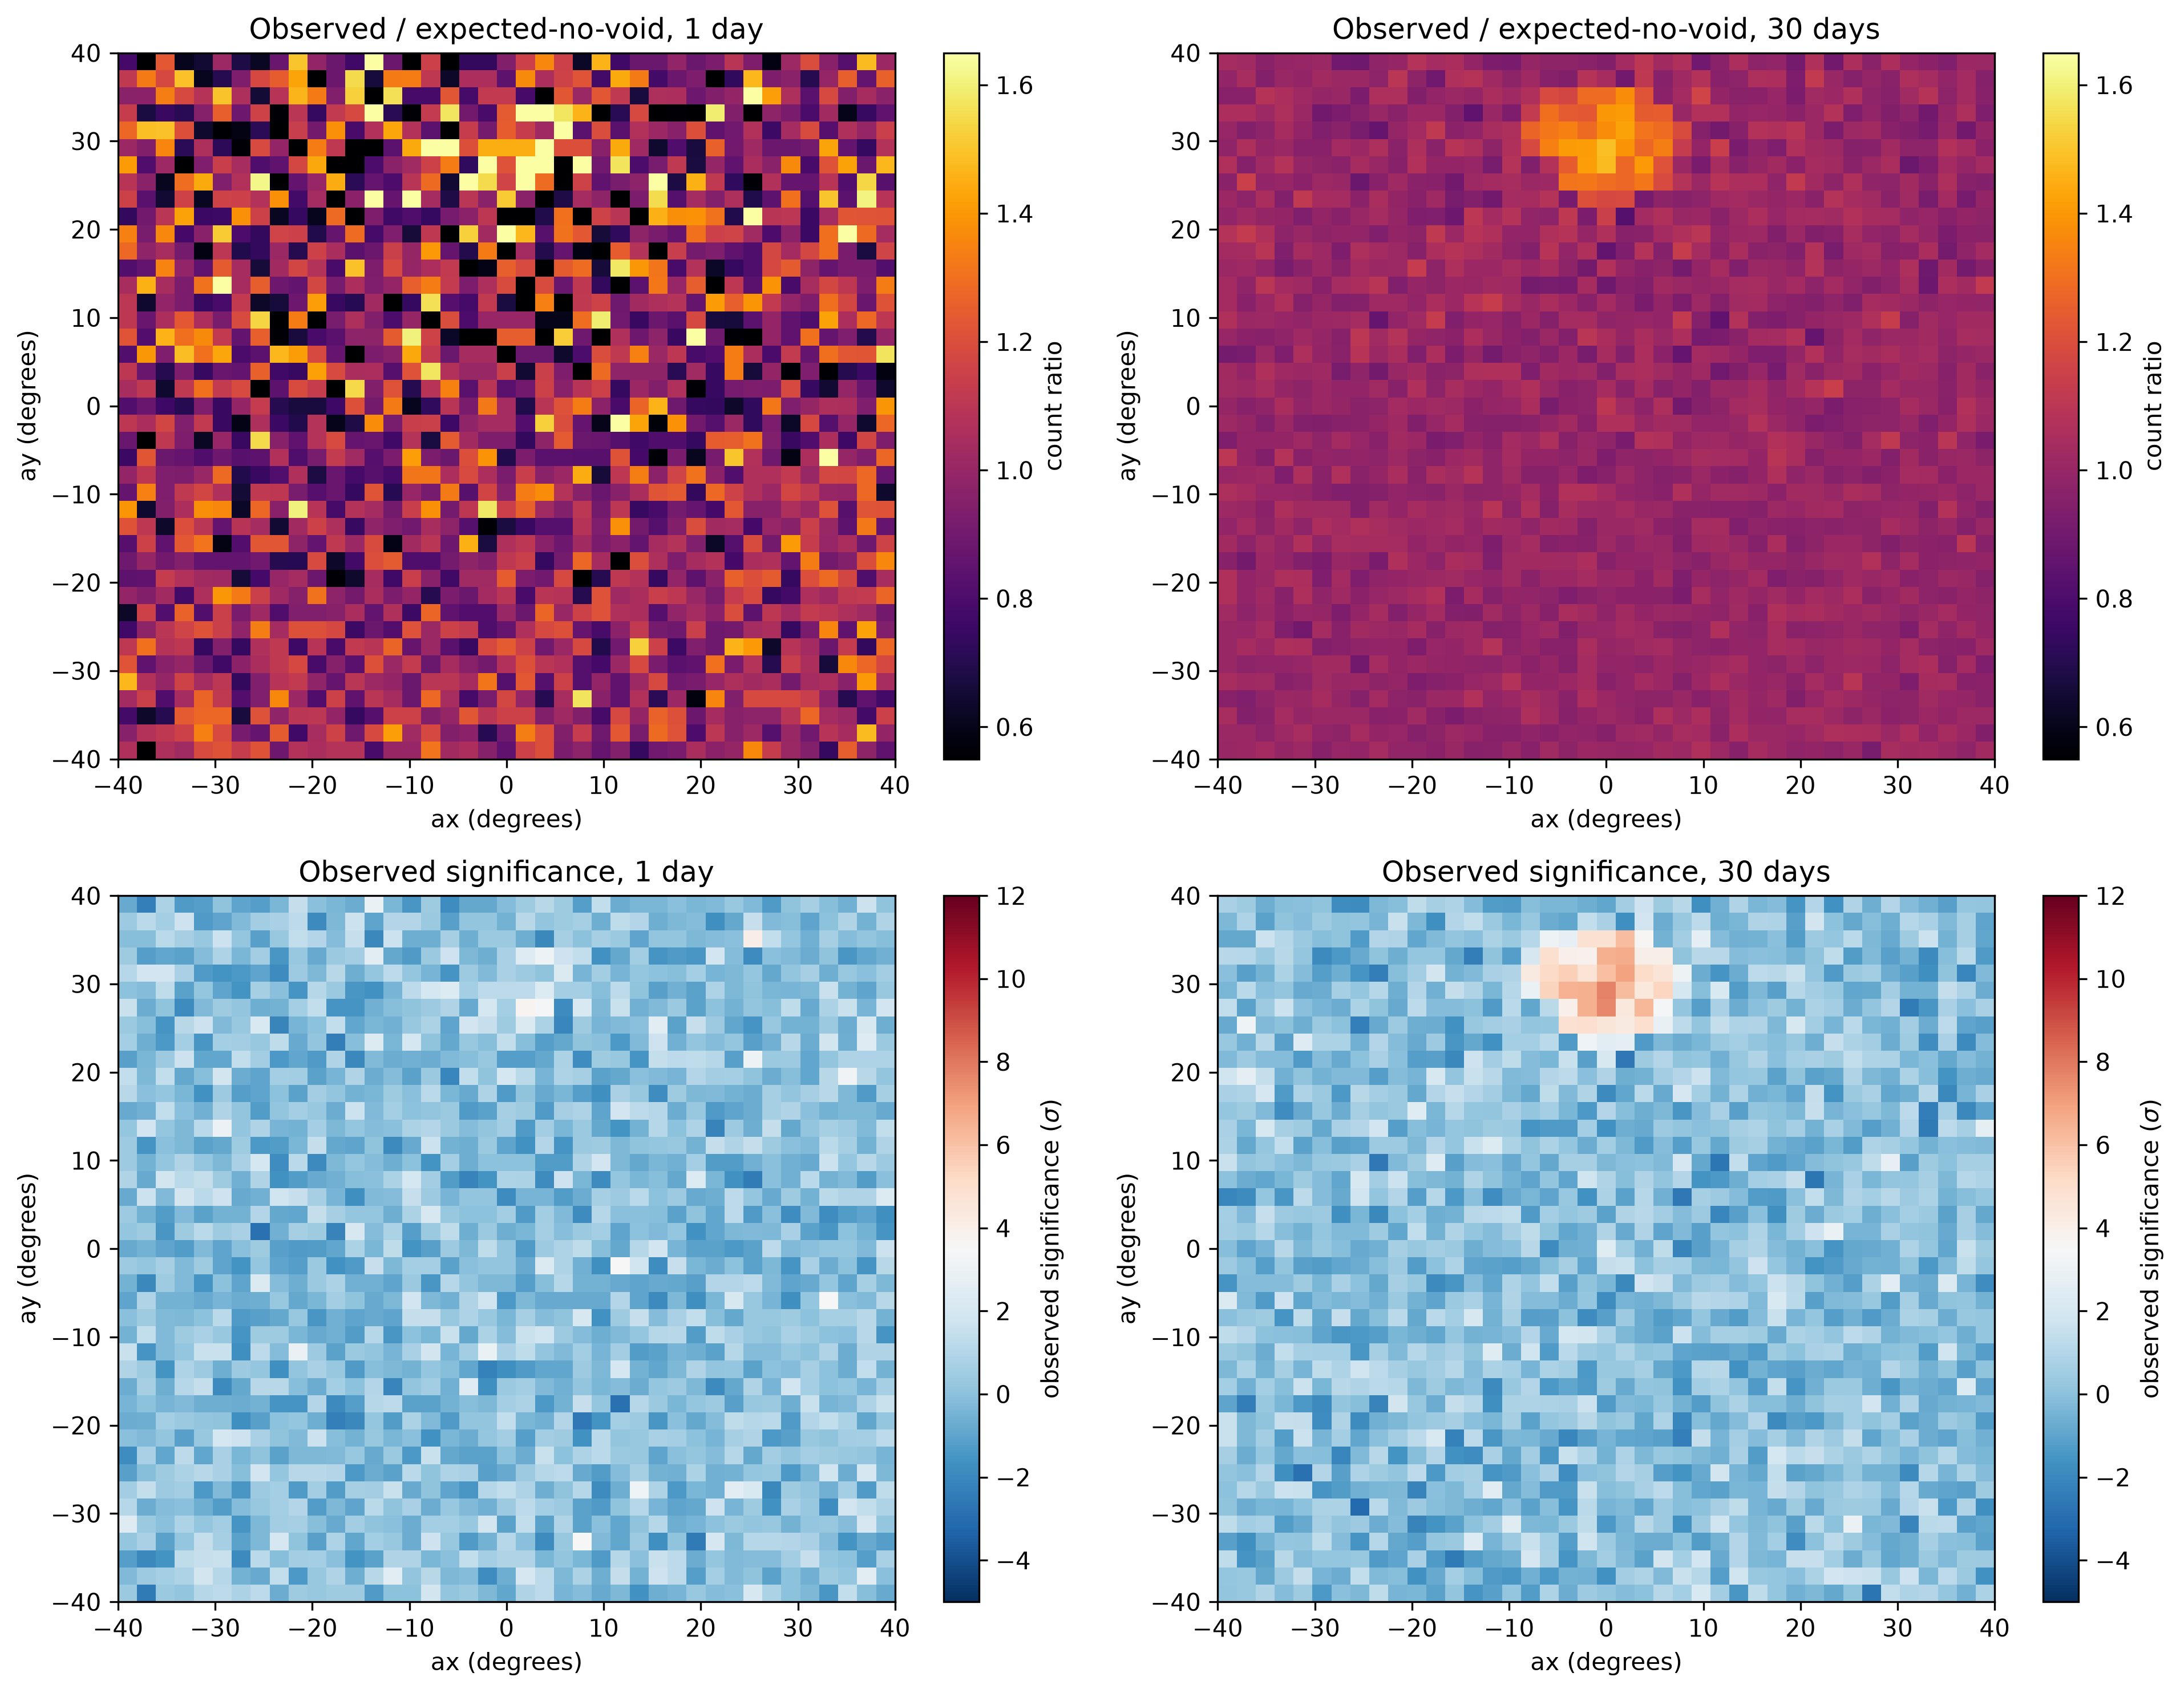
\includegraphics[width=0.78\textwidth]{10_noise_significance.png}
    \caption{Poisson-noisy observations at 1 and 30 days. Top: observed counts
    divided by the no-void expectation. Bottom: observed significance. The
    chamber is invisible at one day and clear at 30 days. Seed 0.}
    \label{fig:noise}
\end{figure}

\begin{figure}[h]
    \centering
    \begin{subfigure}{0.48\textwidth}
        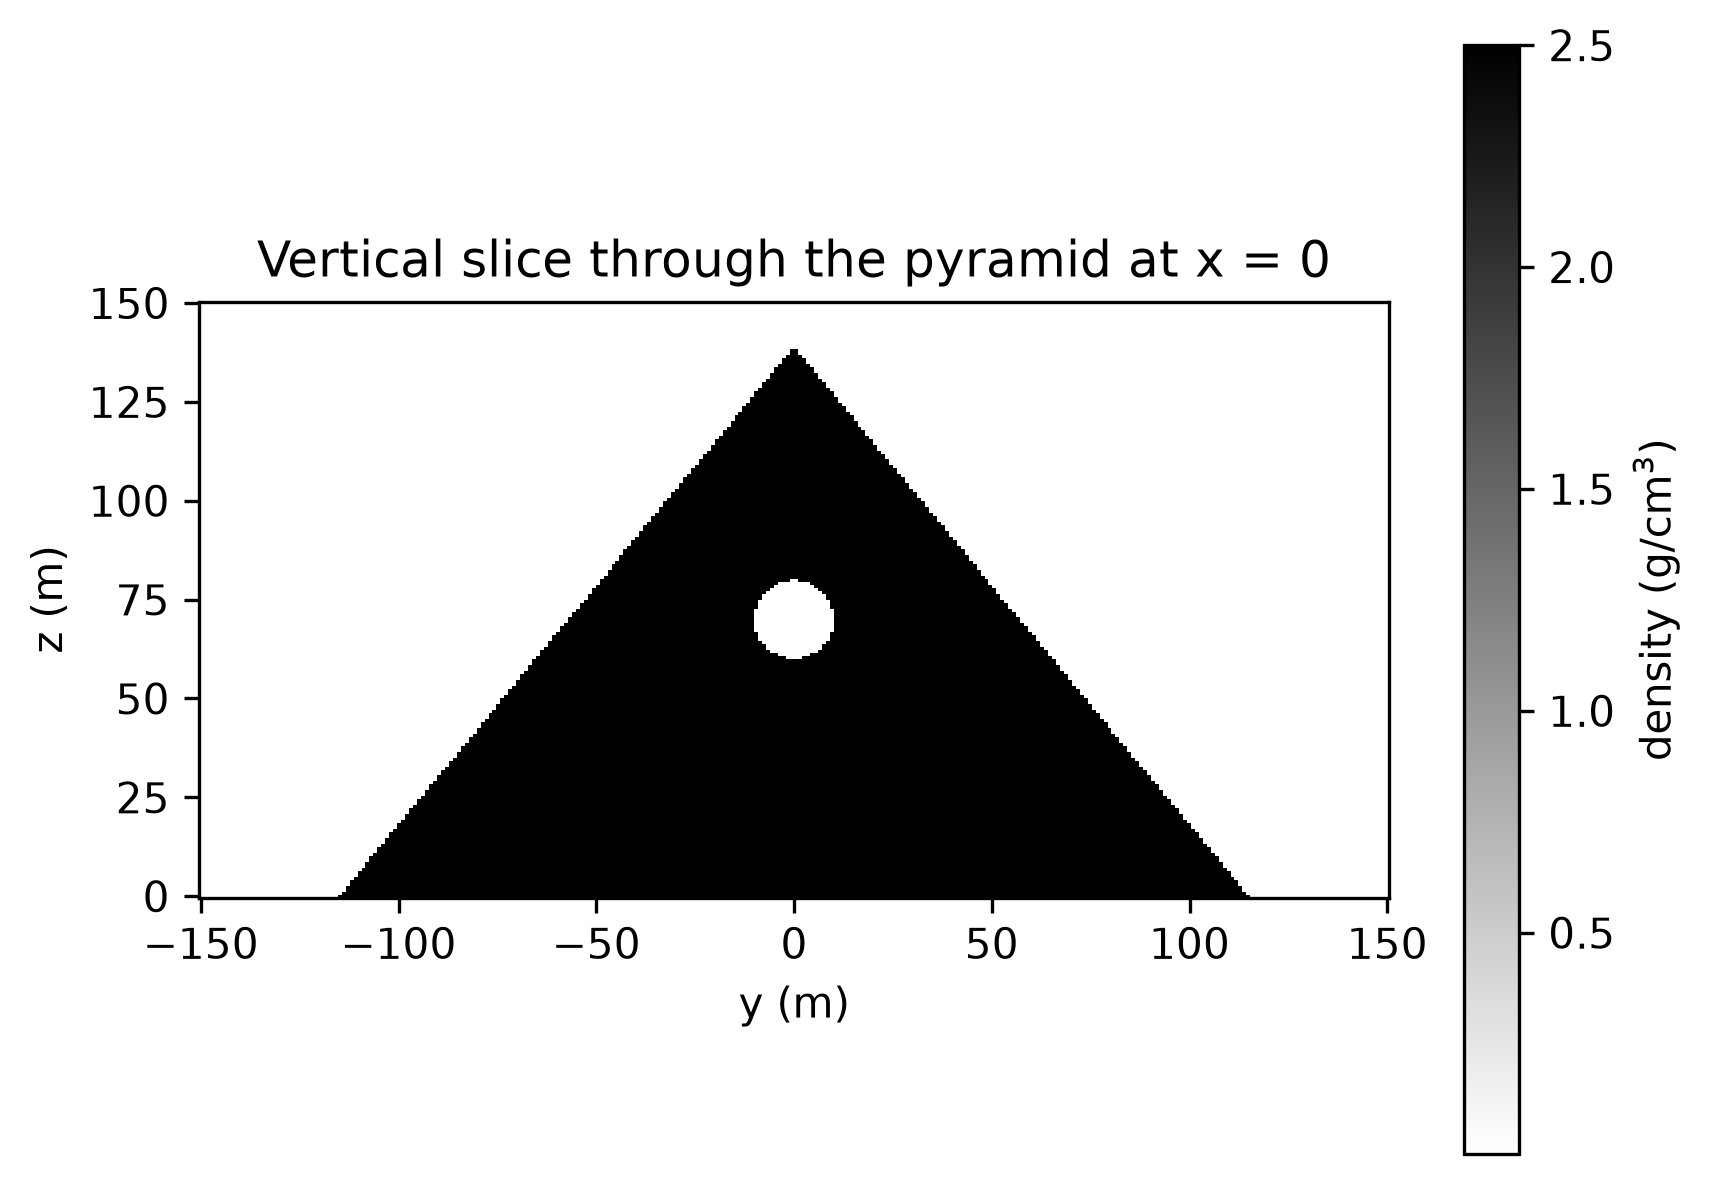
\includegraphics[width=\linewidth]{05_density_slice.png}
        \caption{Density slice at $x=0$. The chamber is the circular air-filled
        region at $z=70$~m.}
        \label{fig:densityslice}
    \end{subfigure}\hfill
    \begin{subfigure}{0.48\textwidth}
        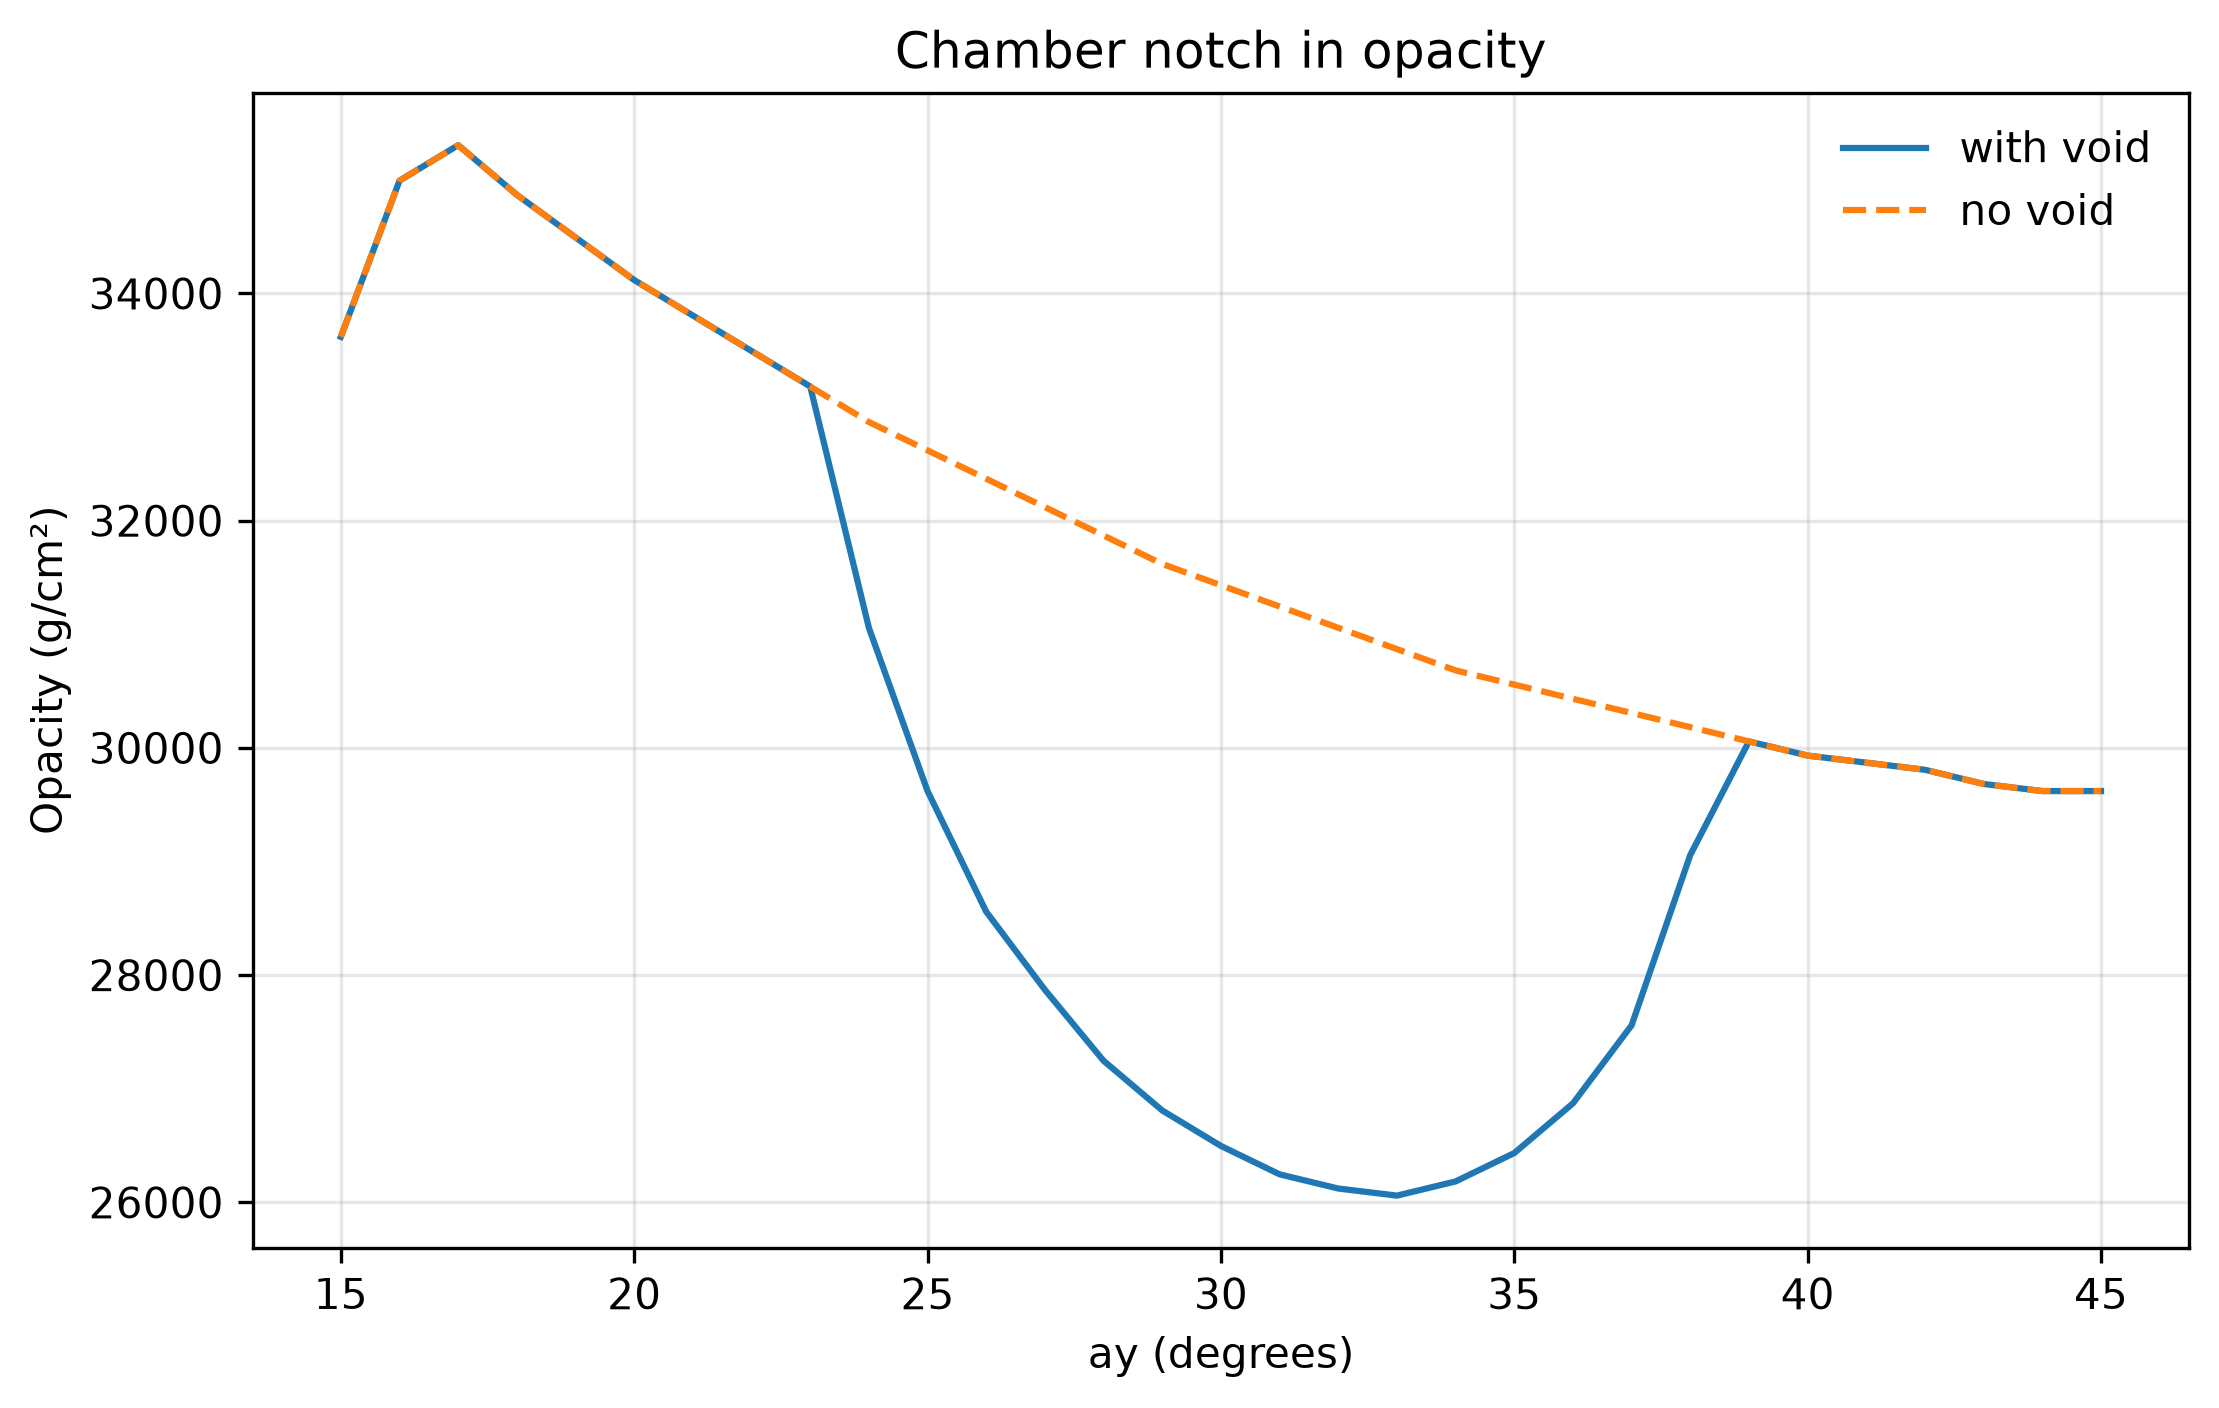
\includegraphics[width=\linewidth]{06_opacity_notch.png}
        \caption{Opacity versus vertical pointing angle at $a_x=0^\circ$ with
        and without the chamber. The notch is the chamber signature.}
        \label{fig:notch}
    \end{subfigure}
    \caption{The target and its first ray-traced signature. The chamber lowers
    the opacity by about $4{,}900$~g\,cm$^{-2}$; the no-void control is flat.}
    \label{fig:target}
\end{figure}



\begin{figure}[h]
    \centering
    \begin{subfigure}{0.48\textwidth}
        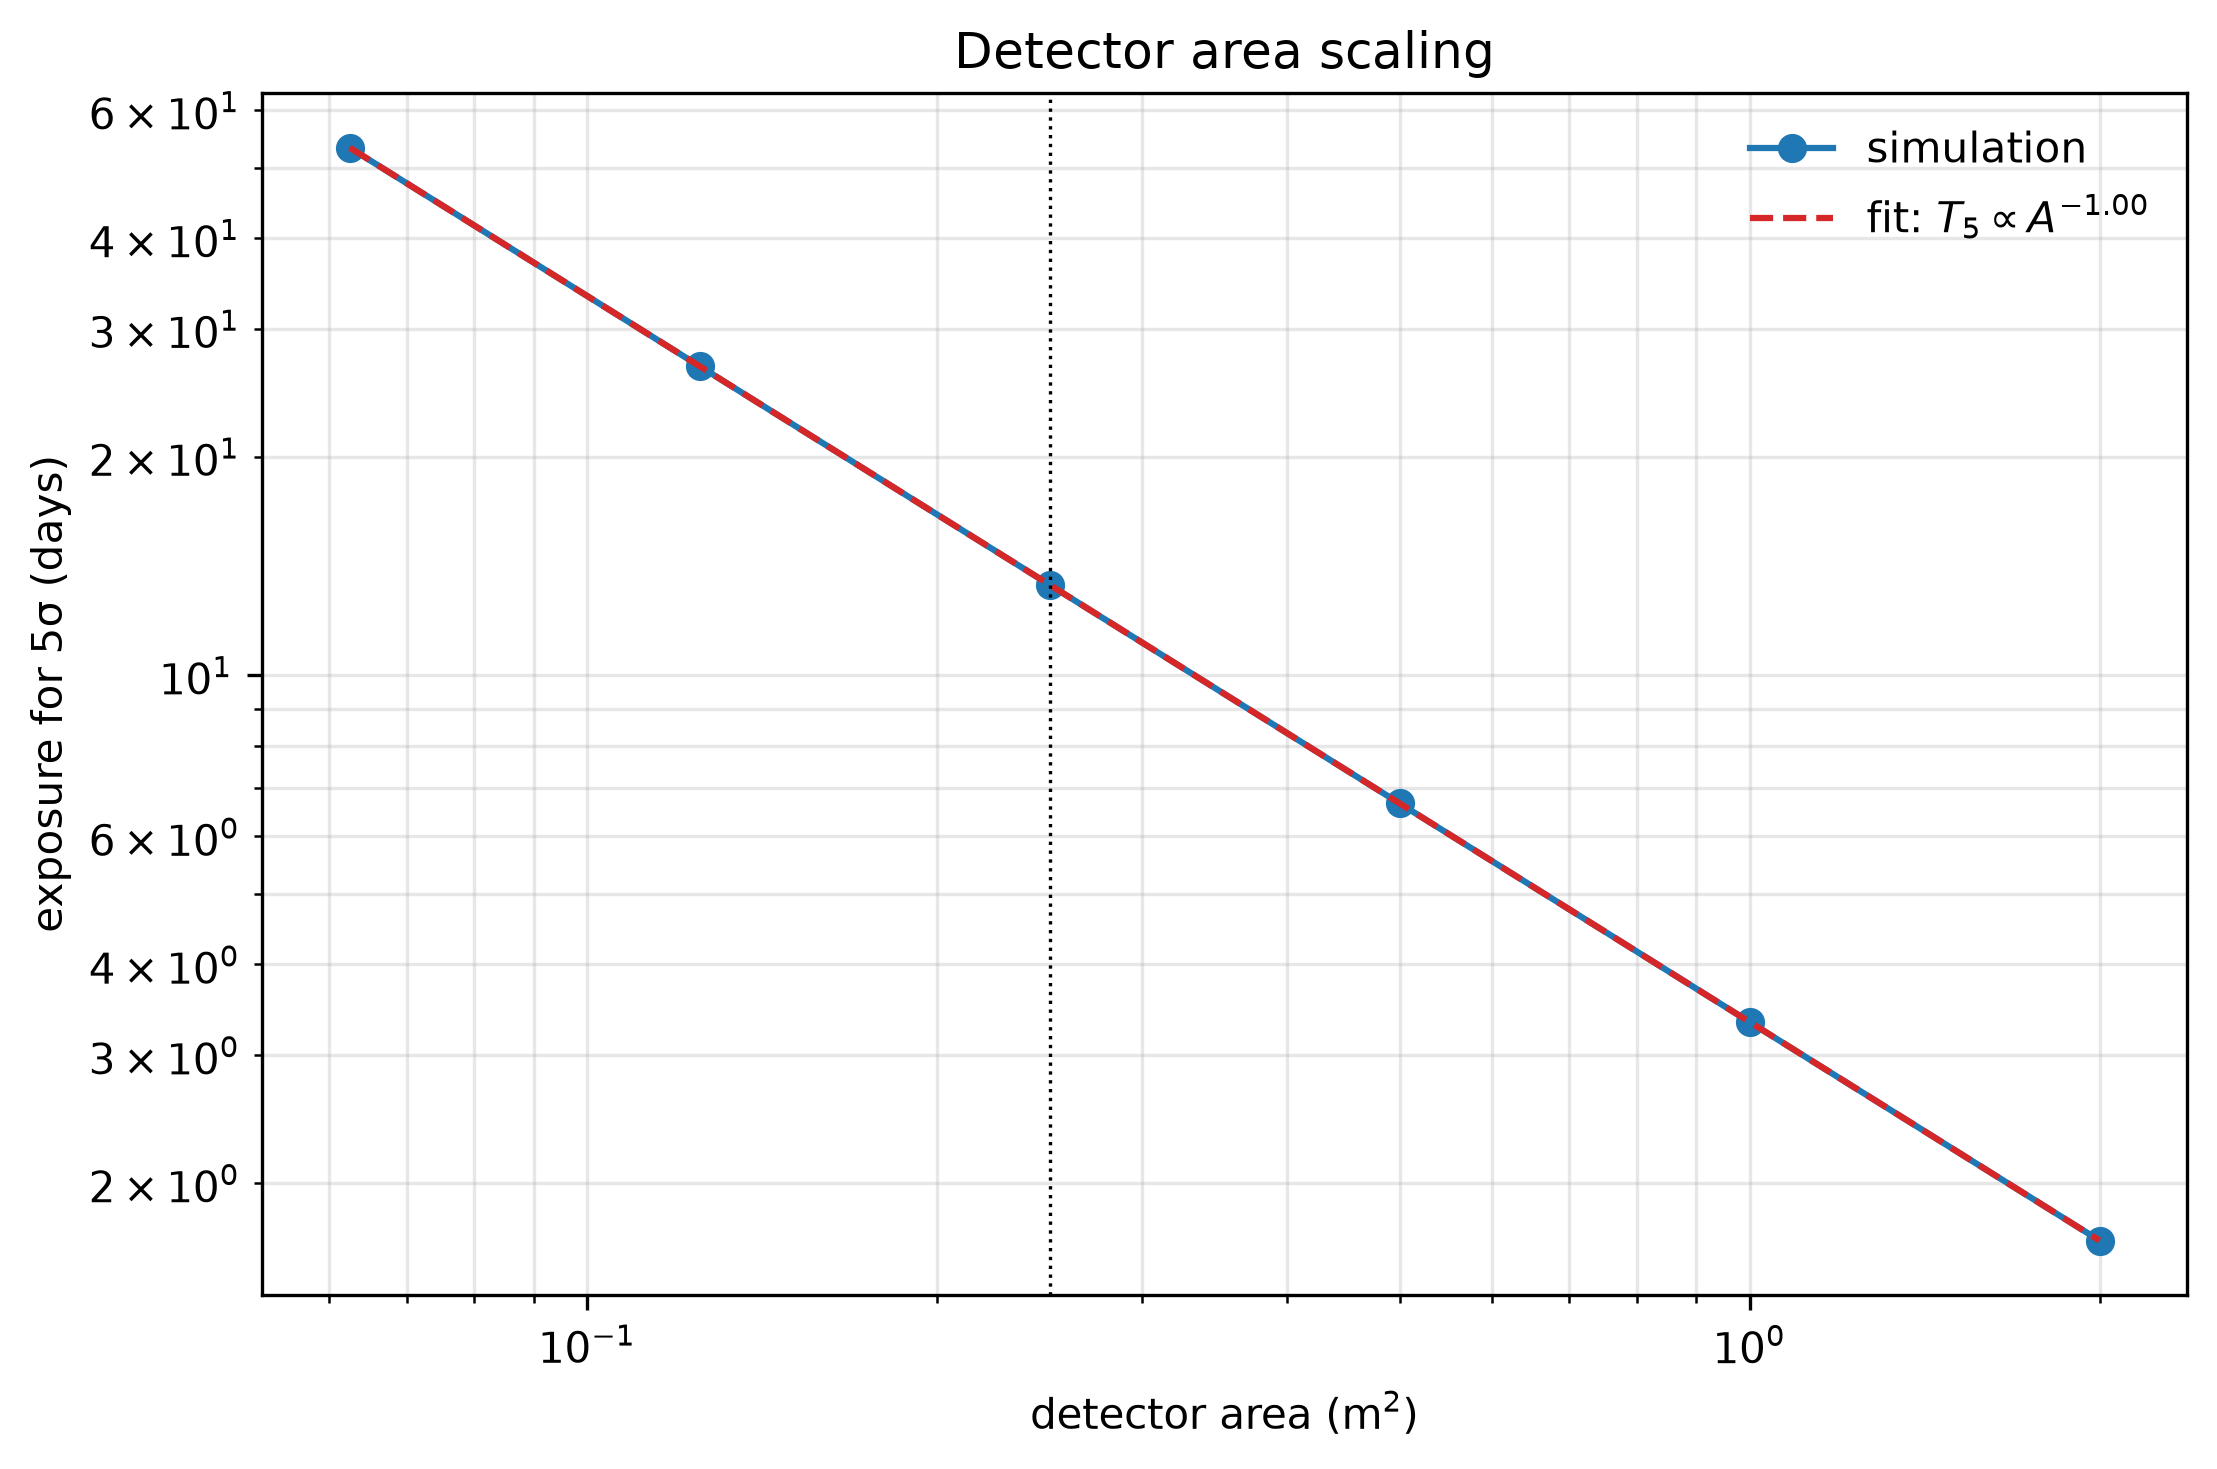
\includegraphics[width=\linewidth]{20_area_scaling.png}
        \caption{Detector-area scaling. The fit is $T_5\propto A^{-1.00}$.}
        \label{fig:area}
    \end{subfigure}\hfill
    \begin{subfigure}{0.48\textwidth}
        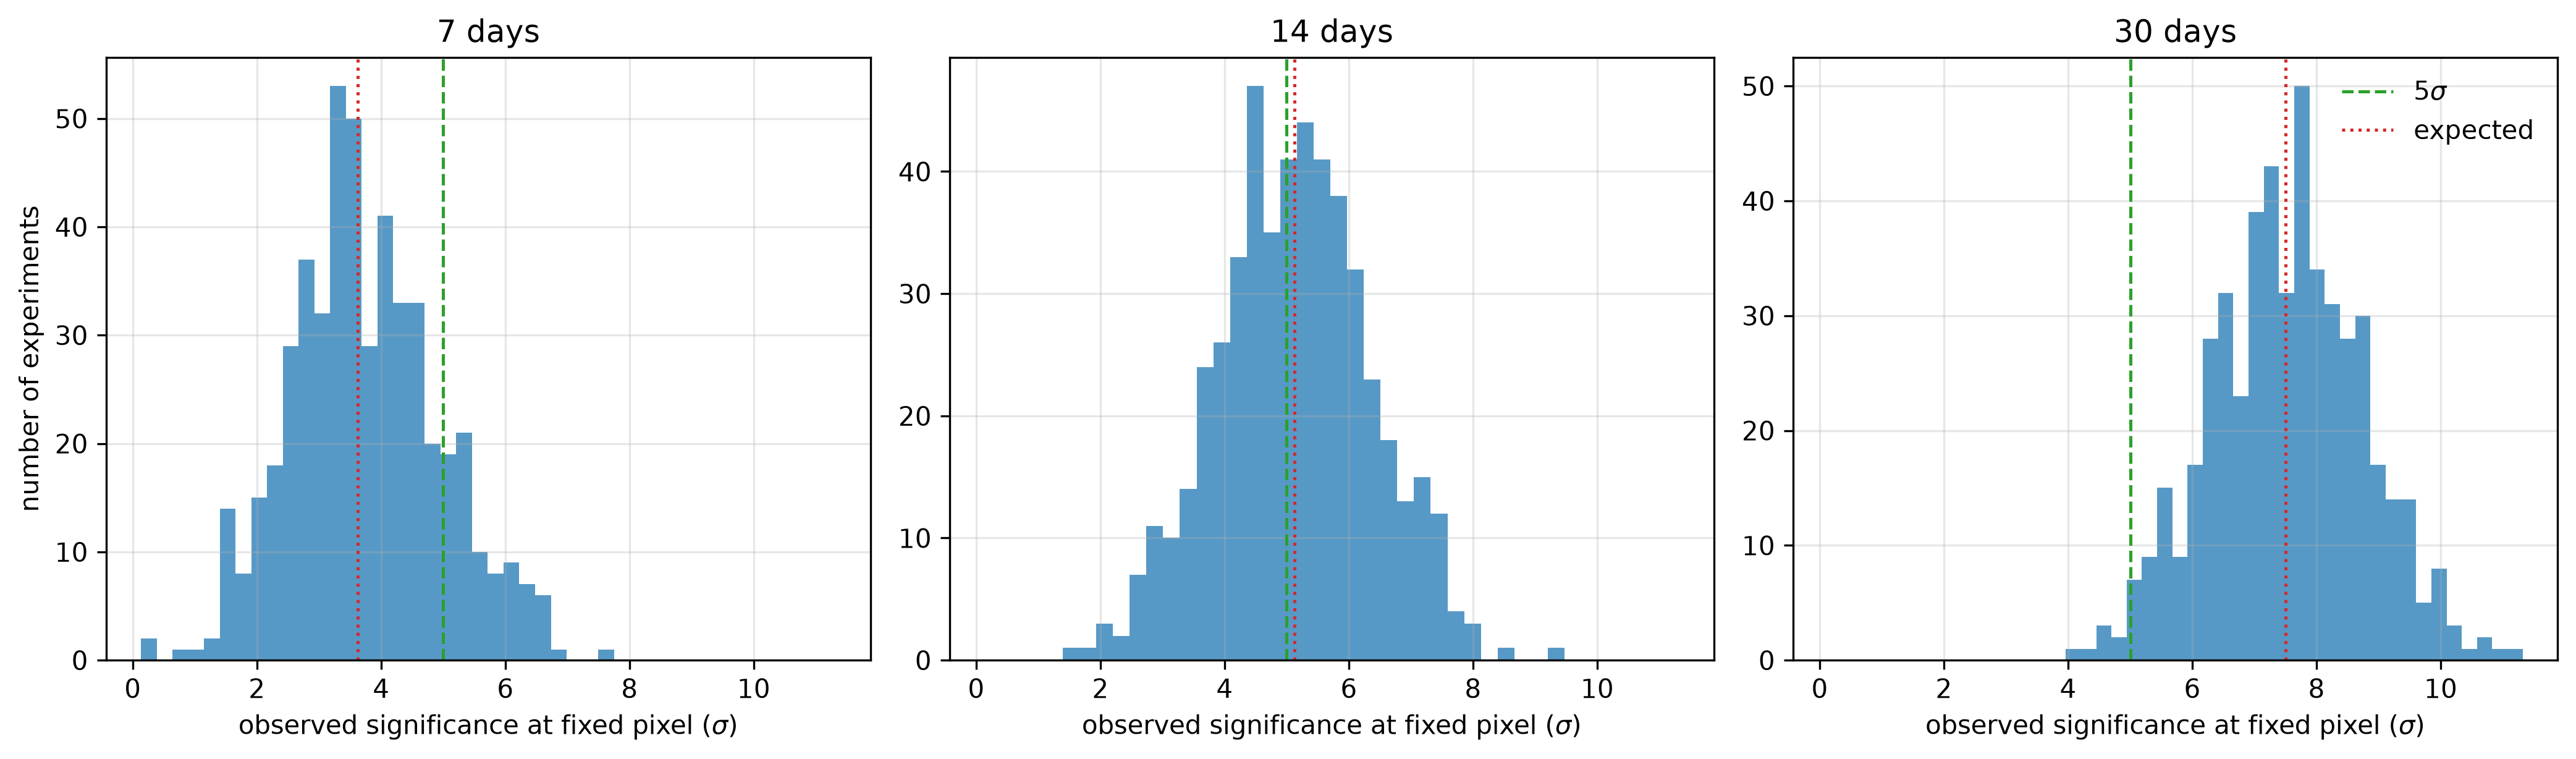
\includegraphics[width=\linewidth]{13_observed_distribution.png}
        \caption{Observed significance at the fixed pixel for 7, 14 and 30
        days, 500 experiments each.}
        \label{fig:dist}
    \end{subfigure}
    \caption{Supplementary checks: detector-area scaling and the fluctuation
    of a real observation around the expected curve.}
    \label{fig:supp}
\end{figure}

\begin{figure}[h]
    \centering
    \begin{subfigure}{0.58\textwidth}
        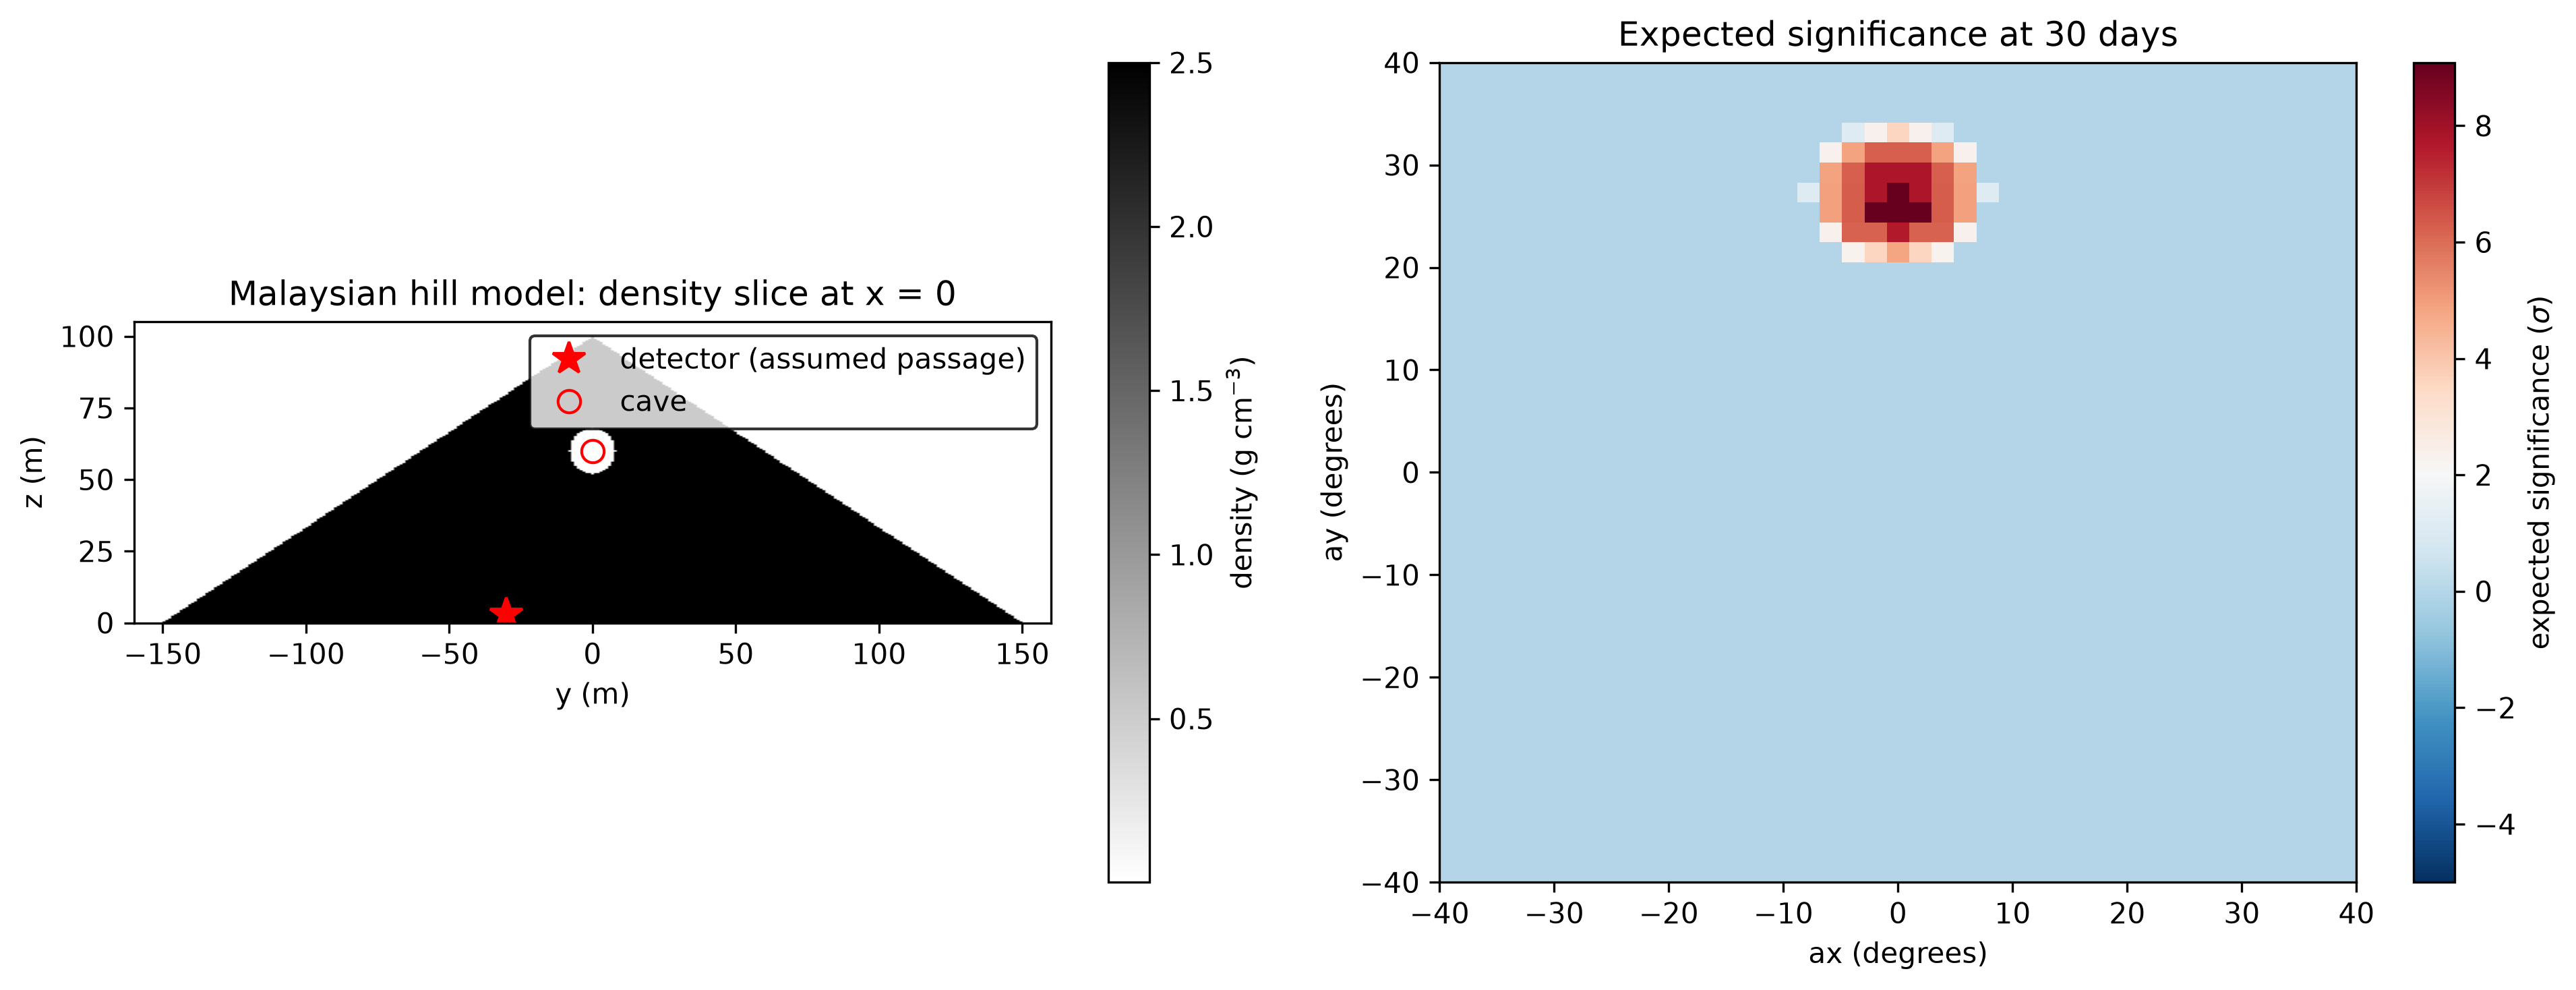
\includegraphics[width=\linewidth]{18_malaysian_target.png}
        \caption{Hypothetical Malaysian hill: density slice and expected
        significance at 30 days.}
        \label{fig:malaysian}
    \end{subfigure}\hfill
    \begin{subfigure}{0.40\textwidth}
        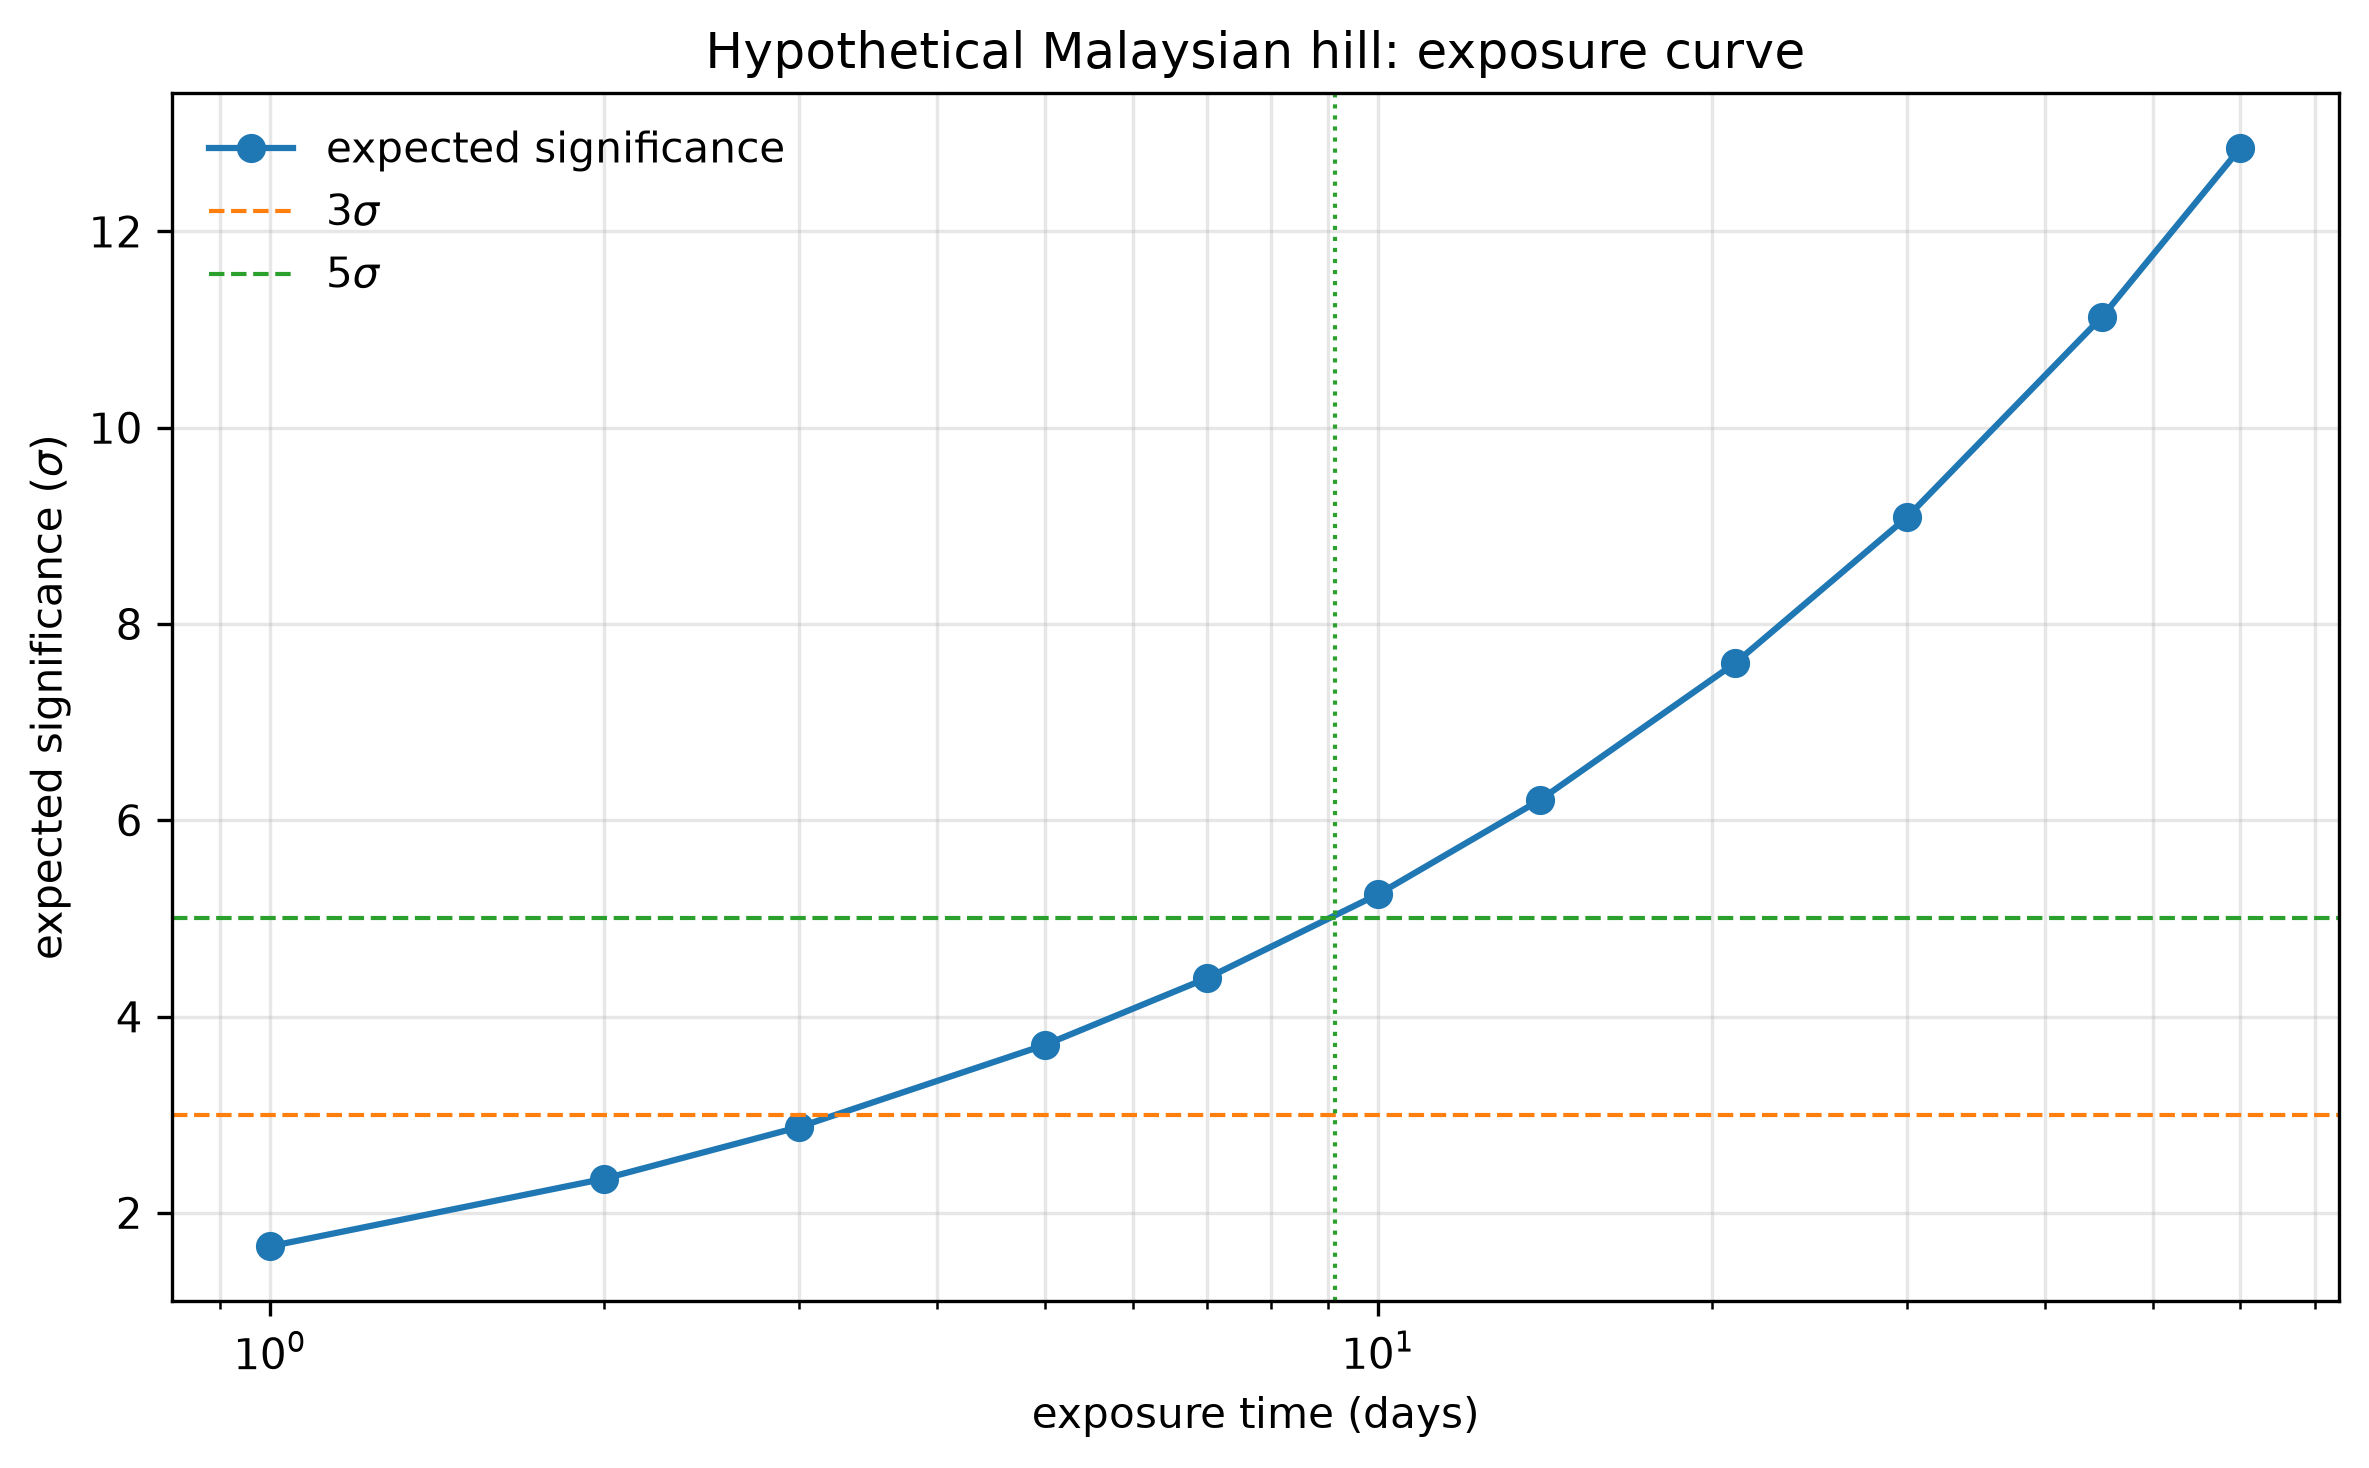
\includegraphics[width=\linewidth]{19_malaysian_exposure.png}
        \caption{Exposure curve for the same hill; $5\sigma$ at 9.1 days.}
        \label{fig:malaysianexp}
    \end{subfigure}
    \caption{The hypothetical Malaysian limestone-hill extension. This is a
    toy target, not a survey of a real site.}
    \label{fig:malaysianfig}
\end{figure}

\begin{figure}[h]
    \centering
    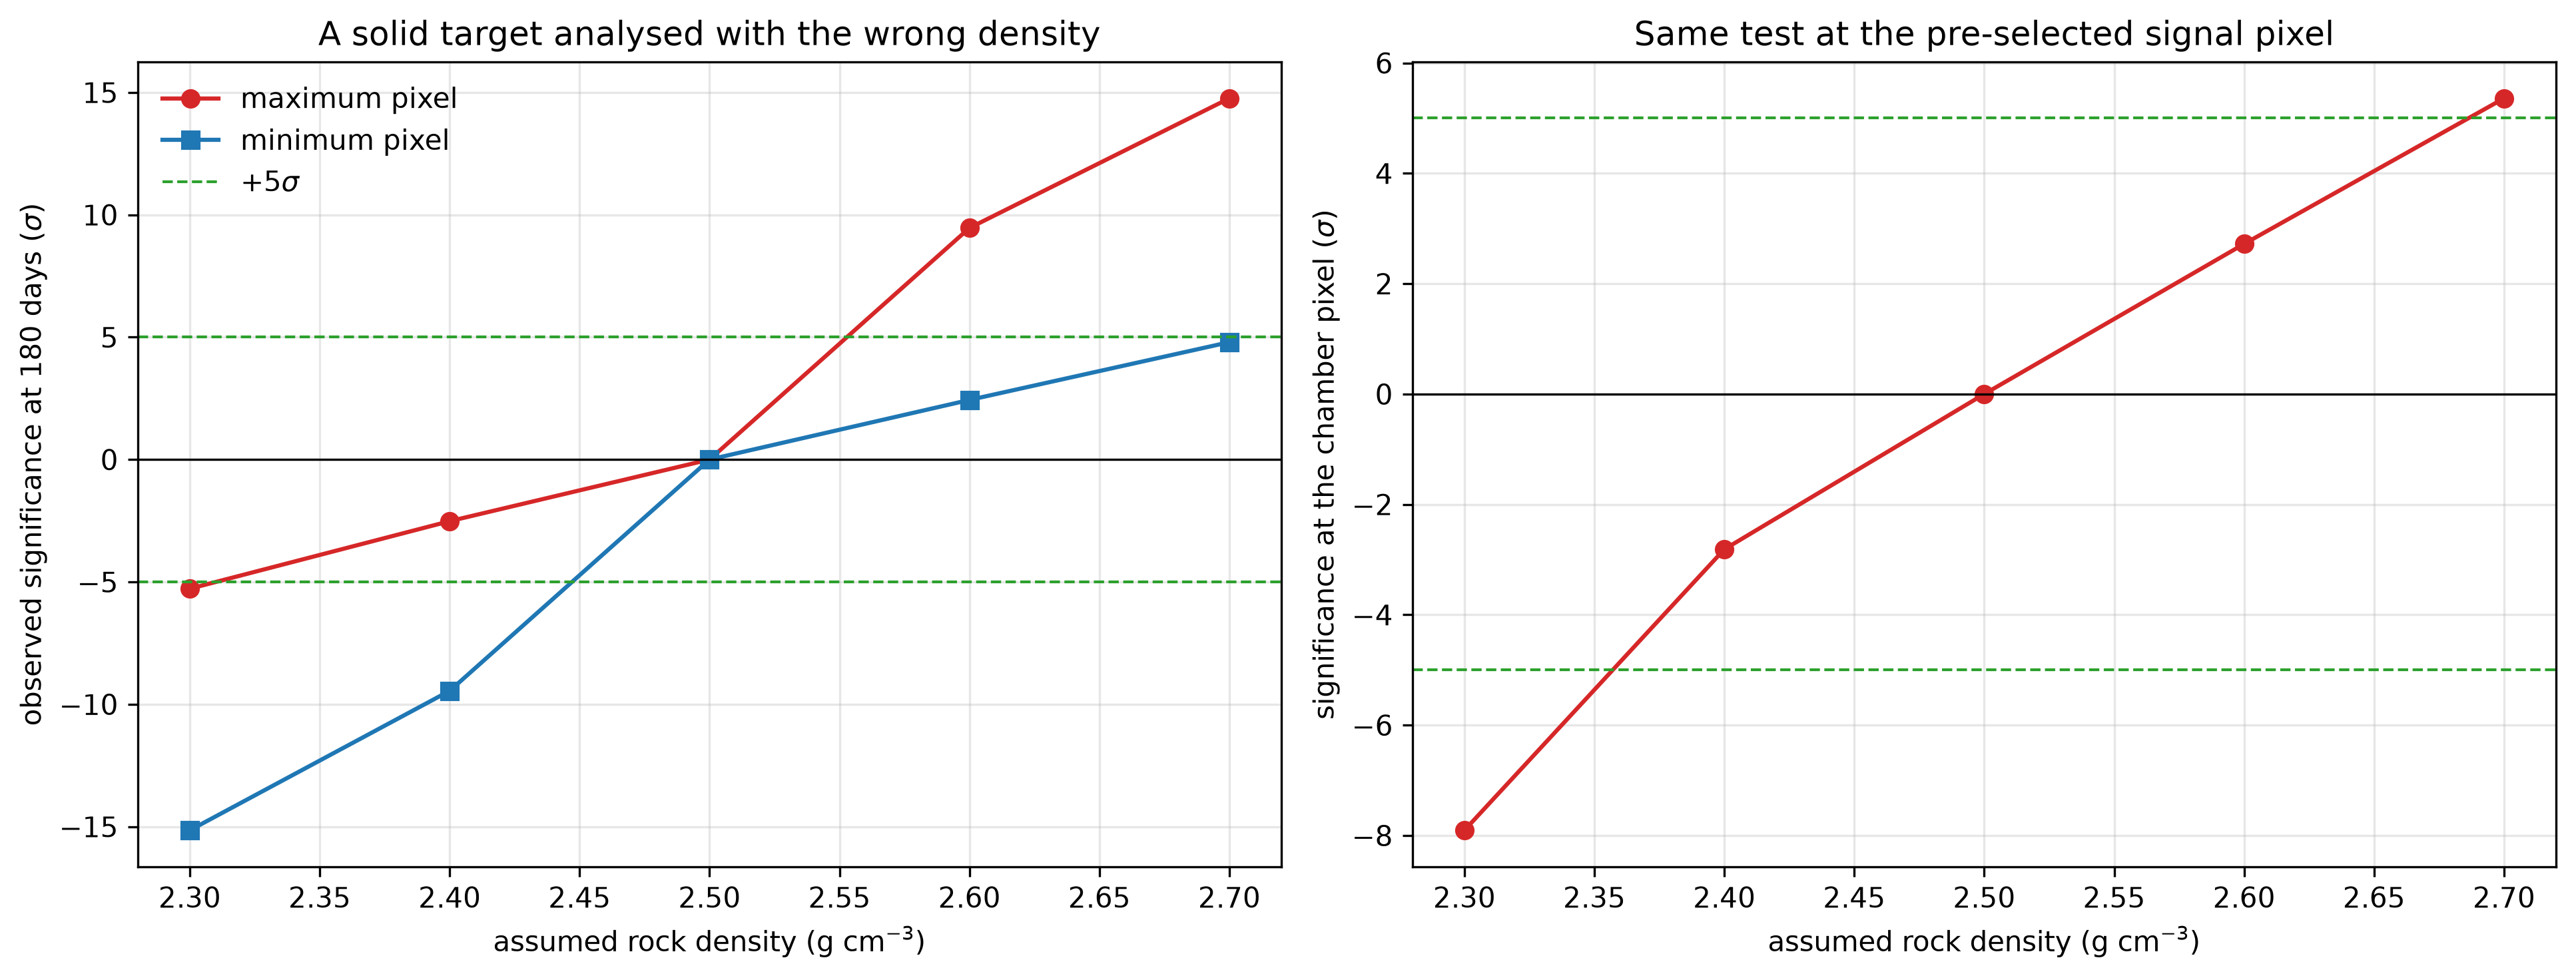
\includegraphics[width=0.78\textwidth]{21_density_systematics.png}
    \caption{Density systematics. A solid target is analysed with the wrong
    assumed density. A 4\% error produces a fake maximum above $5\sigma$ by
    180 days, and the fake signal follows the shape of the target.}
    \label{fig:densitysys}
\end{figure}

\begin{figure}[h]
    \centering
    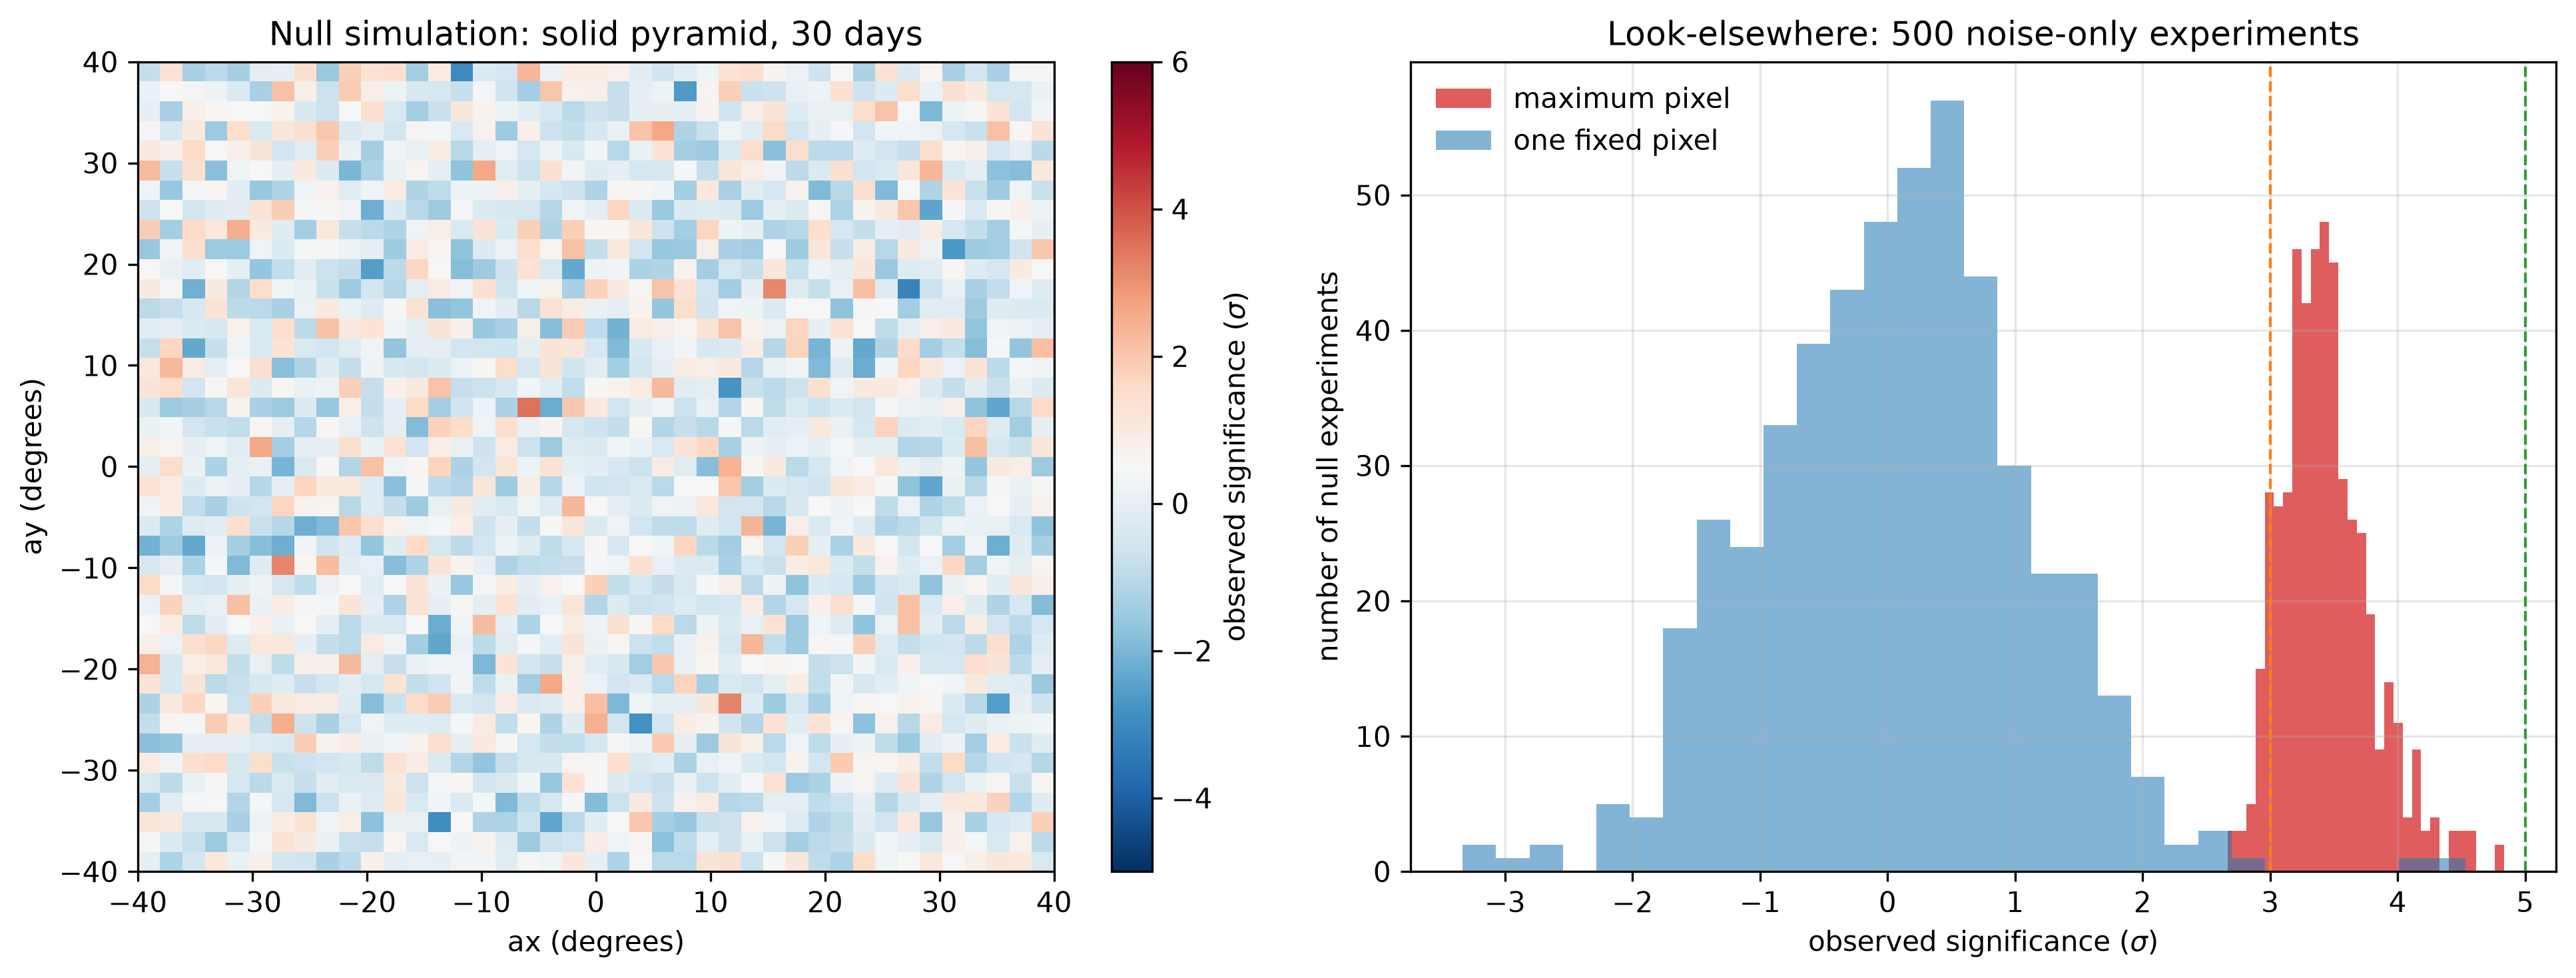
\includegraphics[width=0.78\textwidth]{12_null_ensemble.png}
    \caption{The no-void control. Left: one noise-only significance map. Right:
    the distributions of the maximum pixel and one fixed pixel over 500 null
    experiments. The maximum is pushed to $\approx3.4\sigma$ by the number of
    pixels searched.}
    \label{fig:null}
\end{figure}

\begin{figure}[h]
    \centering
    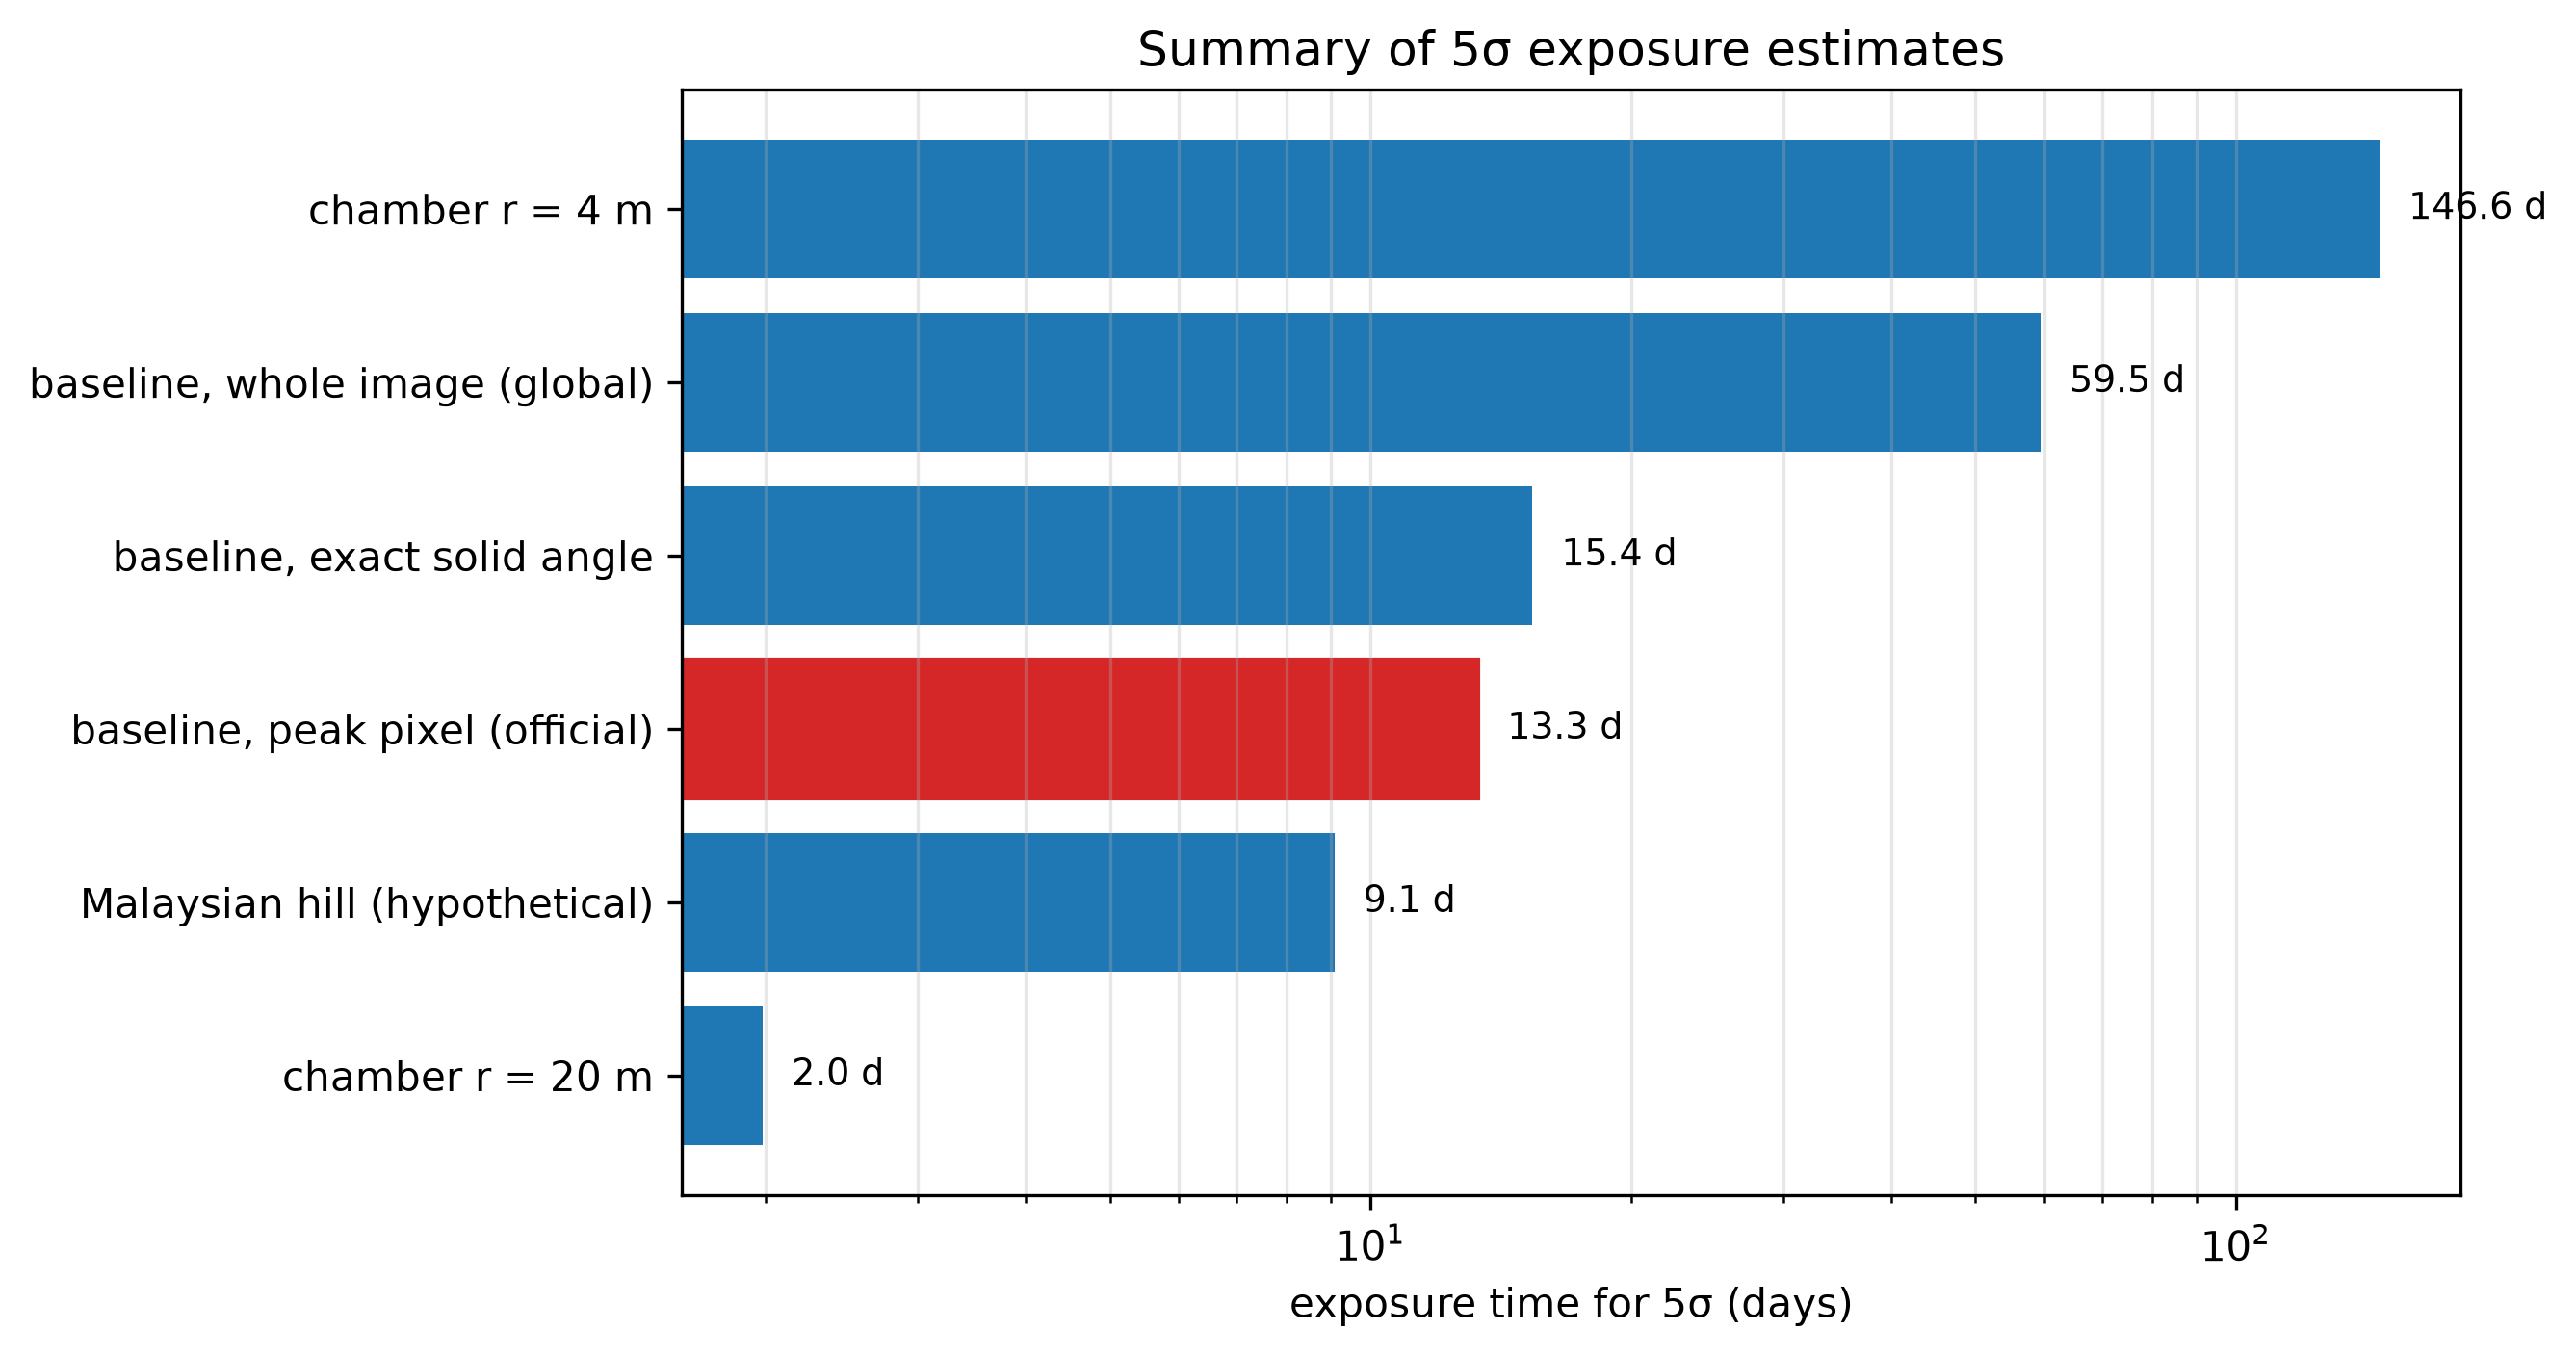
\includegraphics[width=0.70\textwidth]{22_exposure_summary.png}
    \caption{Summary of the $5\sigma$ exposure estimates under different
    definitions and assumptions. The official baseline is highlighted.}
    \label{fig:summary}
\end{figure}

\section{Derivation of the Minimum Survival Energy}
\label{app:derivation}

Starting from
\begin{equation}
\frac{dE}{dX}=-(a+bE),
\end{equation}
separate variables and integrate from $E=E_{\min}$ at $X=0$ to $E=0$ at
$X=\varrho$:
\begin{equation}
\int_{E_{\min}}^{0}\frac{dE}{a+bE}=-\int_{0}^{\varrho}dX.
\end{equation}
With $u=a+bE$, $du=b\,dE$, the left side is
\begin{equation}
\frac{1}{b}\ln\left(\frac{a}{a+bE_{\min}}\right)=-\varrho,
\end{equation}
so
\begin{equation}
E_{\min}(\varrho)=\frac{a}{b}\left(e^{b\varrho}-1\right).
\end{equation}
For small $b\varrho$, $e^{b\varrho}-1\approx b\varrho$ and
$E_{\min}\approx a\varrho$. At $\varrho=25{,}000$~g\,cm$^{-2}$ the exact value
is 52.59~GeV, 5.2\% above the linear 50~GeV.

\section{Code Availability}
\label{app:code}

\begin{sloppypar}
The repository is \texttt{evan-student-package/}. The figure-to-notebook mapping
is given in Table~\ref{tab:code}. The shared analysis functions are in
\texttt{code/student\_analysis.py}; the baseline parameters are in
\texttt{code/project\_config.py}; the summary of all numbers is
\texttt{figures/results\_summary.json}. Notebooks 03--05 import the shared
module and run from a fresh kernel.
\end{sloppypar}

\begin{table}[h]
\centering
\caption{Figure-to-notebook mapping.}
\label{tab:code}
\small
\begin{tabular}{@{}ll@{}}
\toprule
Figure(s) & Notebook \\
\midrule
Fig.~\ref{fig:physics} & \texttt{01\_muons\_and\_rock.ipynb} \\
Fig.~\ref{fig:target} & \texttt{02\_ray\_tracing.ipynb} \\
Fig.~\ref{fig:image} & \texttt{03\_first\_image.ipynb} \\
Figs.~\ref{fig:noise}, \ref{fig:exposure} & \texttt{04\_noise\_and\_exposure.ipynb} \\
Figs.~\ref{fig:studies} and Appendix figures & \texttt{05\_parameter\_study.ipynb} \\
\bottomrule
\end{tabular}
\end{table}

\end{document}

